\documentclass[
	%sans,			% use sans-serif font
	%serif,			% use serif-font
	%mathsans,		% set mathtext to sans-serif
	%mathserif,		% set mathtext to serif
	%10pt,
	10pt,
	%12pt,
	t		% add text at the top border of slide
	%slidescentered,% center text on slide
	%draft,			% compile as draft version
	%handout,		% create handout file
	%notes,			% include nodes in slides
	%compress		% compress navigation bar
]{beamer}

\usetheme{lmtslides}
\usepackage{eso-pic}
\usepackage{graphicx}
%\usepackage[pdftex]{color}
\usepackage{times}
\usepackage[latin1]{inputenc}
%\usepackage[T1]{fontenc}
\usepackage[amssymb]{SIunits}
\usepackage{amsmath,amssymb}
\usepackage{eurosym}
\usepackage{booktabs}
\usepackage{colortbl}
\usepackage{url}
\usepackage[absolute,overlay]{textpos}
\usepackage{graphicx}
\usepackage{mathtools}
\usepackage{pifont}% http://ctan.org/pkg/pifont
\usepackage{appendixnumberbeamer}
\usepackage{subcaption}

\newcommand{\xmark}{\ding{55}}%
\newcommand{\cmark}{\ding{51}}%

\renewcommand{\footnoterule}{\vfill\kern -3pt  \kern 2.6pt}

\setbeamertemplate{caption}{\raggedright\insertcaption\par}
\setbeamertemplate{bibliography item}[online]
\graphicspath{{figures/}}

\setlang{en}		

% Supervisor: Univ.-Prof. Dr. Hans-Joachim Bungartz
% Advisors: Manish Kumar Mishra, M.Sc. (hons) &
% Samuel James Newcome, M.Sc.

% MODIFY THESE ACCORDINGLY! ---
\title{Exploring Fuzzy Tuning Technique for Molecular Dynamics Simulations in AutoPas}
\type{Bf} % (M/B/D/S)(f/m): (Master/Bachelor/Diplom/Studienarbeit)(final/midterm)
\author{Manuel Lerchner}
\email{manuel.lerchner@tum.de}
\advisorOne{Manish Kumar Mishra, M.Sc.}
\advisorTwo{Samuel James Newcome, M.Sc.}
\date{\today}
%------------------------------



\AtBeginSection[]
{
    \begin{frame}
        \frametitle{Table of Contents}
        \tableofcontents[currentsection,currentsubsection]
    \end{frame}
}

%%%%%%%%%%%%%%%%%%%%%%%%%%
\begin{document}

\maketitle

\setcounter{framenumber}{0}

\section{Introduction}
\begin{frame}
	\frametitle{What is AutoPas?}
	
	\begin{textblock*}{5cm}(9cm,1.8cm)
		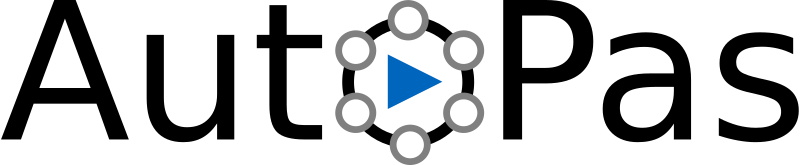
\includegraphics[width=3cm]{figures/AutoPasLogo}
	\end{textblock*}
	
	\begin{itemize}
		\item Library for arbitrary N-body simulations
		\item Optimal performance by switching implementations
		      \begin{itemize}
			      \item \textbf{Container:} Finding neighboring particles
			      \item \textbf{Traversal:} Parallel force calculations
			      \item \textbf{Data Layout:} Memory access optimization
			      \item \textbf{Newton 3:} Force calculation optimization
		      \end{itemize}
	\end{itemize}
	
	\vspace{-0.1cm}
	\begin{figure}
		\centering
		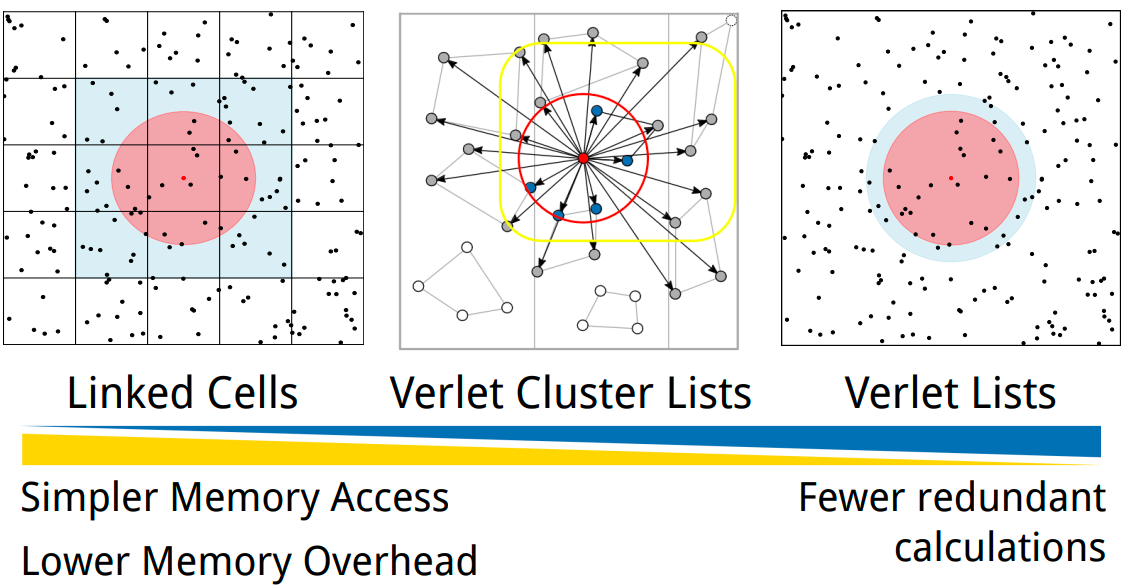
\includegraphics[width=0.72\textwidth]{figures/traversals.png}
	\end{figure}
	
	\begin{textblock*}{5cm}(6.3cm,9.35cm)
		\tiny{\cite{SIAM_PP24}}
	\end{textblock*}
	
\end{frame}


\begin{frame}
	\frametitle{Structure of AutoPas}
	
	\begin{itemize}
		\item Three main areas:
		      \begin{itemize}
			      \item User Application
			      \item Algorithm Library
			      \item Tuning Strategies
		      \end{itemize}
		\item Algorithm Library:
		      \begin{itemize}
			      \item Huge Search Space\footnote{\scriptsize{$\text{Container}\times\text{Traversal} \times \text{Data Layout} \times \text{Newton 3} \times \text{Load Estimator} \times \text{Cell Size Factor}$}
			            }
		      \end{itemize}
		\item Tuning Strategies:
		      \begin{itemize}
			      \item Full Search
			      \item Random Search
			      \item Predictive Tuning
			      \item Bayesian Search
			      \item Rule Based Tuning
		      \end{itemize}
	\end{itemize}
	
	\begin{textblock*}{4cm}(8cm,2cm)
		\begin{figure}
			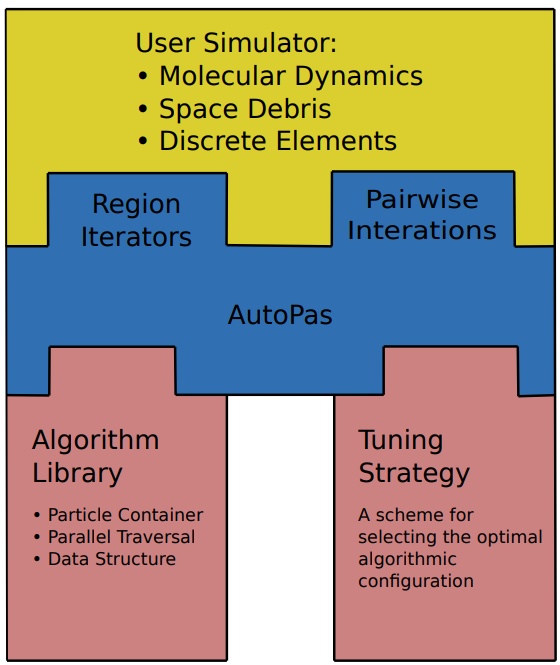
\includegraphics[width=4cm]{figures/AutoPasLibraryStructure.png}
			\caption{ \footnotesize{Source: \cite{Newcome2023Poster}}}
			
		\end{figure}
	\end{textblock*}
\end{frame}



\begin{frame}
	\frametitle{Auto-Tuning }
	
	\begin{itemize}
		\item Tuning Phase $\rightarrow$ Simulation Phase $\rightarrow$ Repeat
		\item Potential Tuning Overhead
	\end{itemize}
	
	\vspace{0.1cm}
	
	\begin{figure}
		\makebox[\textwidth][c]{
			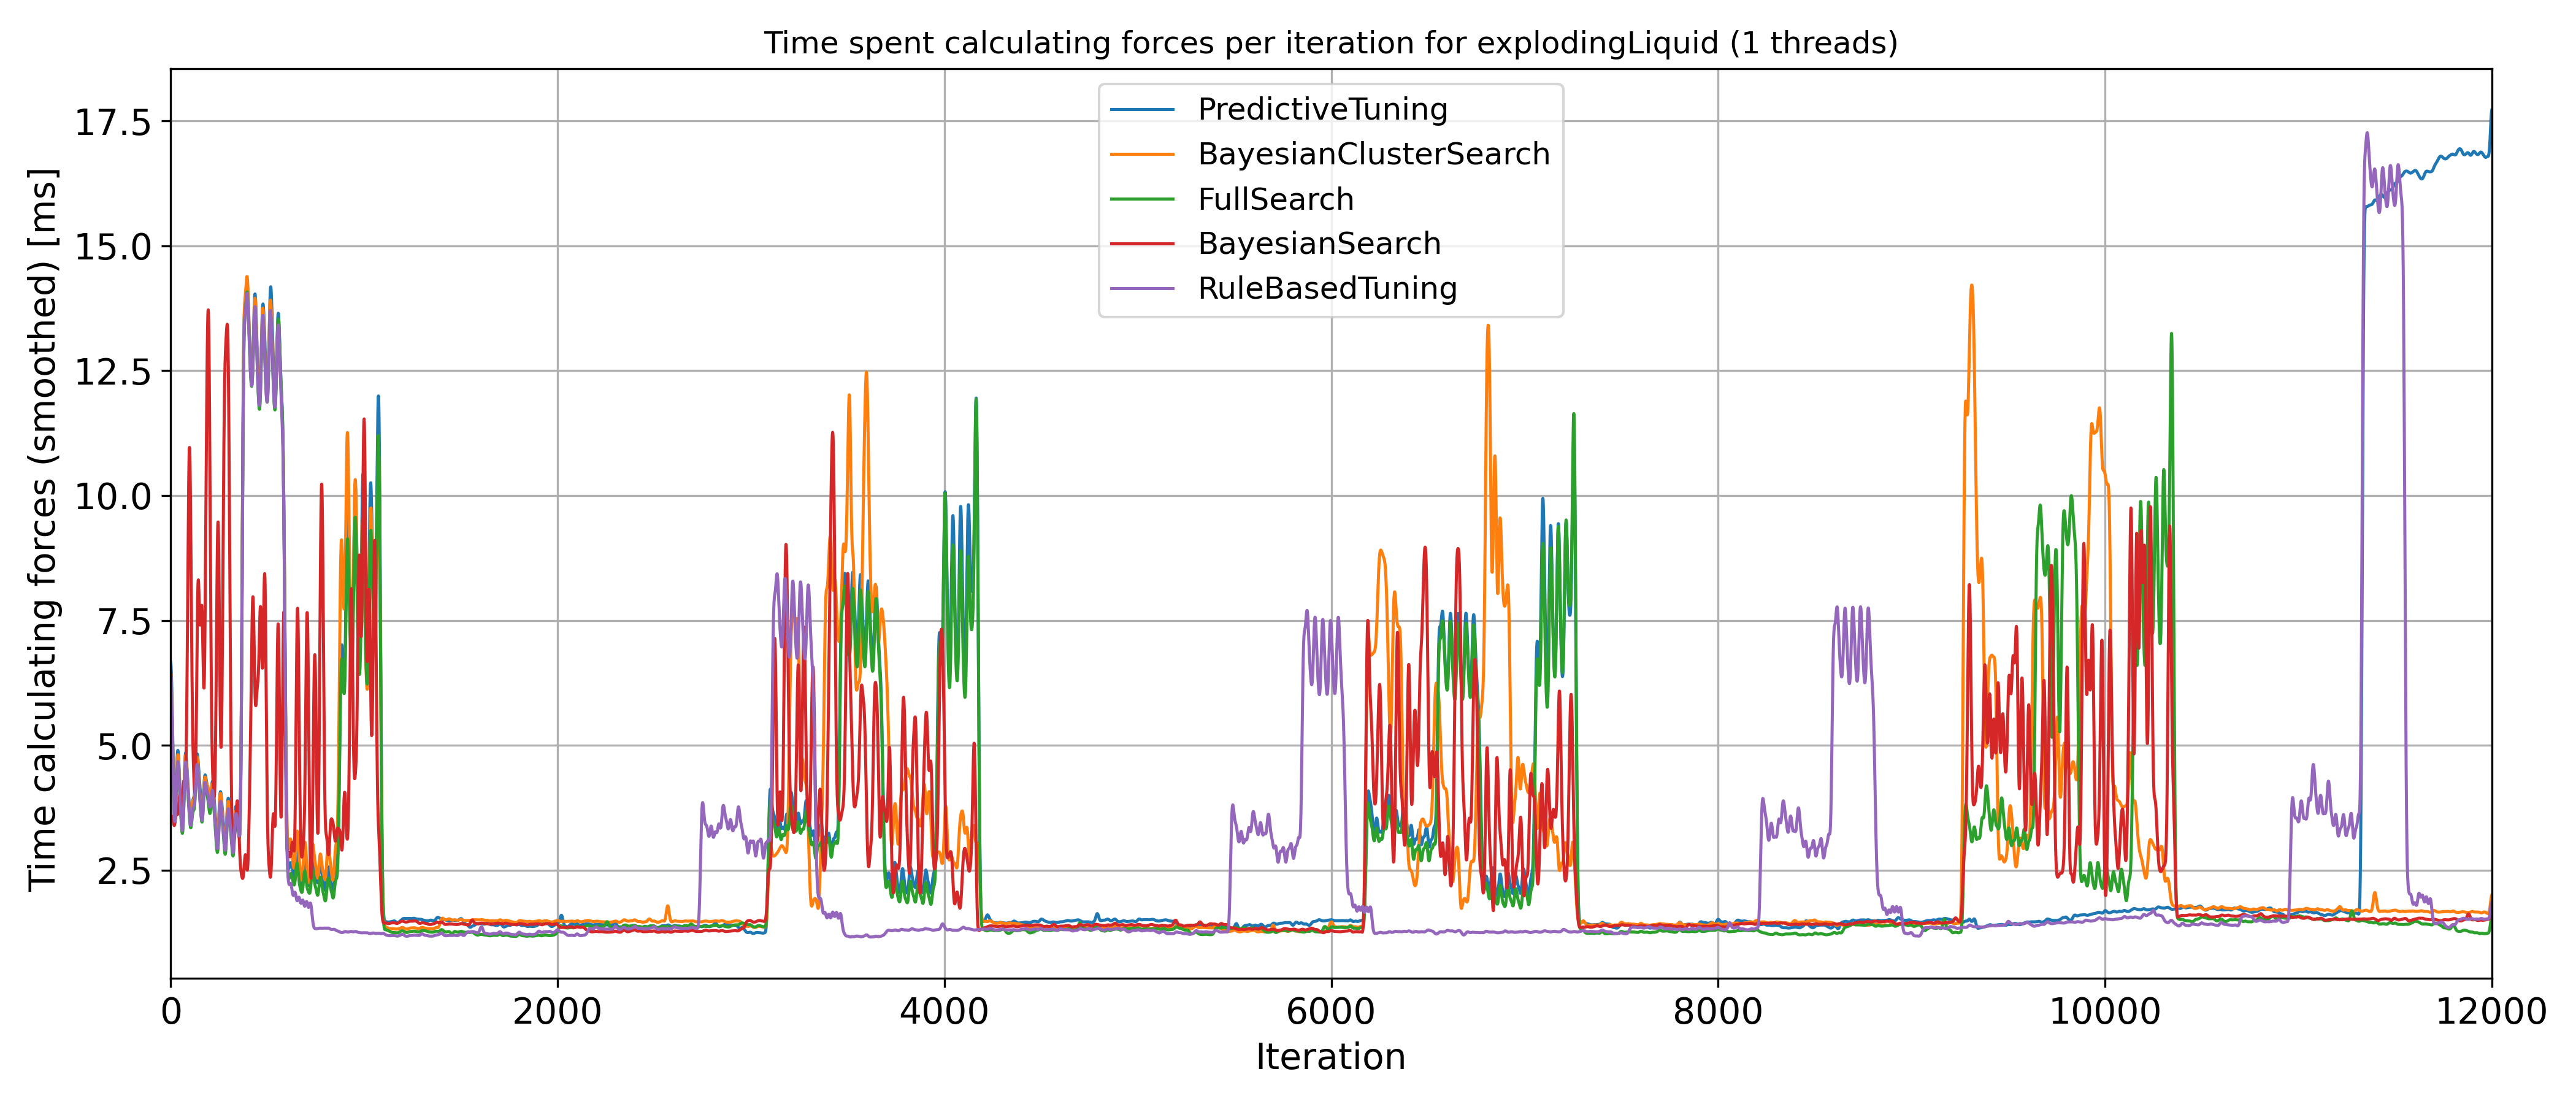
\includegraphics[width=1.1\textwidth,trim={0 0 0 0.85cm},clip]{figures/timing_explodingLiquid.png}
		}
	\end{figure}
	
	
\end{frame}

\begin{frame}
	\frametitle{Idea: Tuning based on Simulation State}
	
	\vspace{-0.4cm}
	
	\begin{figure}
		\centering
		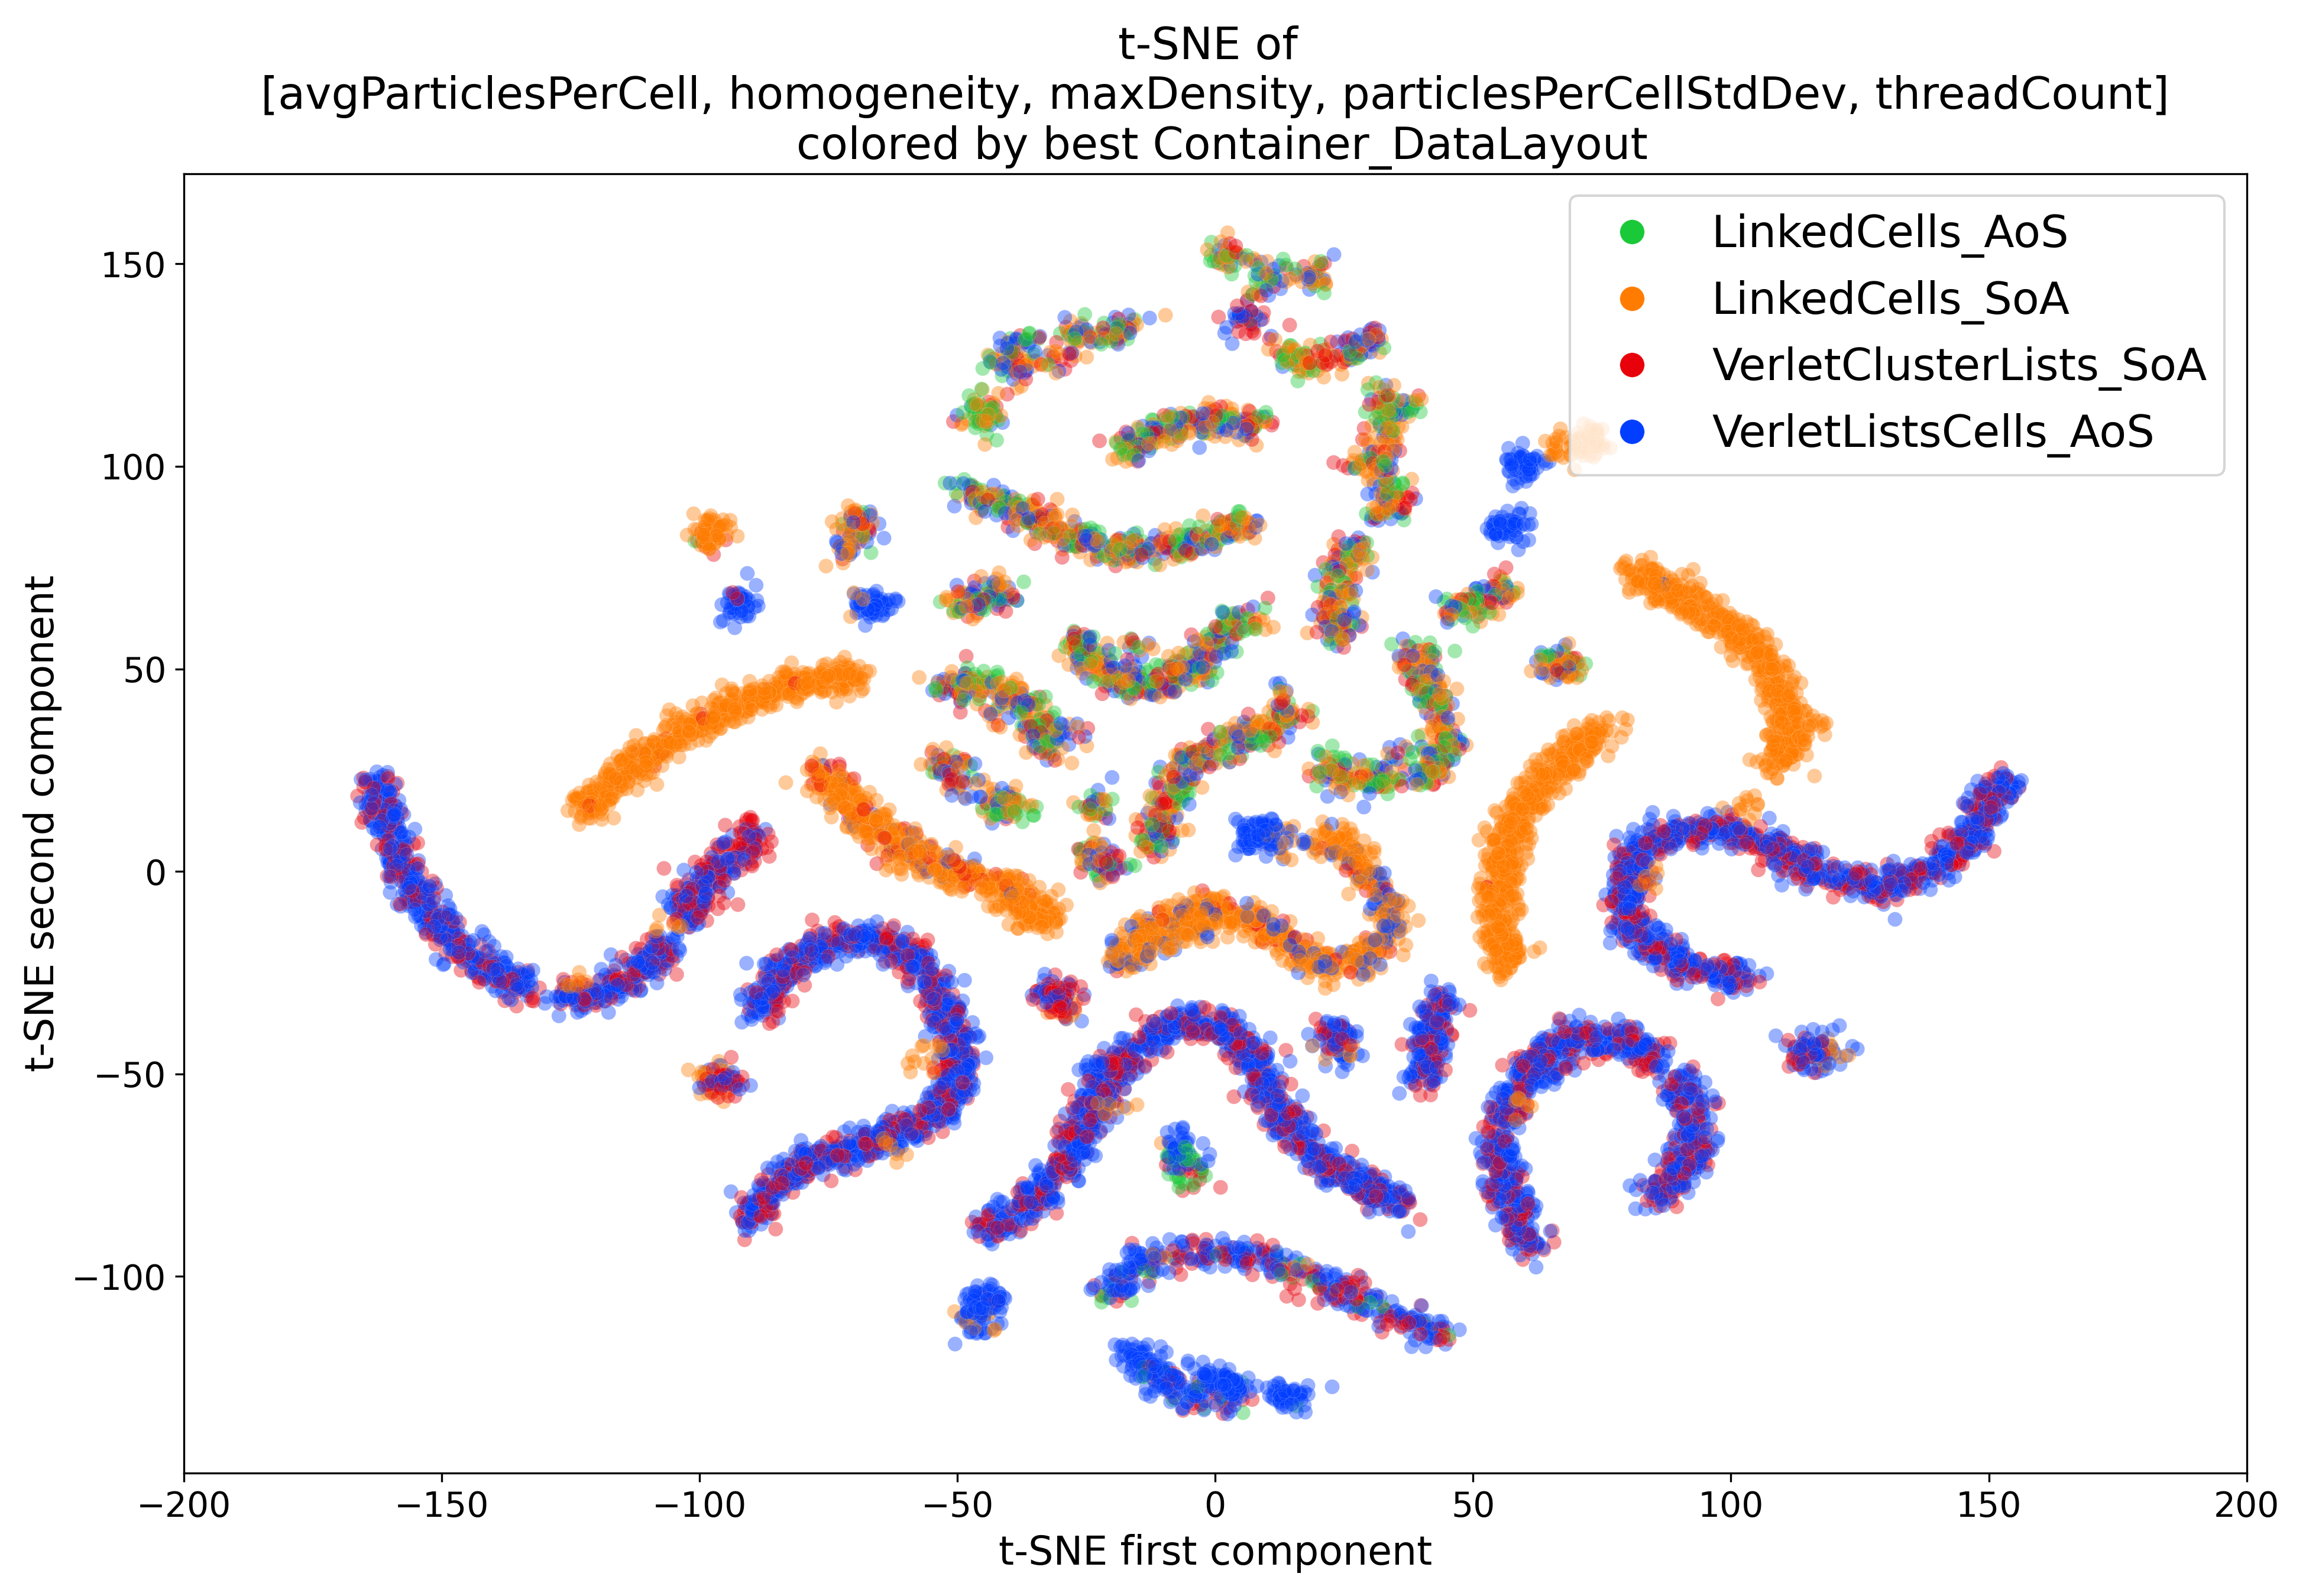
\includegraphics[width=0.9\textwidth,trim={0 0 0 0cm},clip]{figures/t-SNE_Container_DataLayout_filtered.png}
	\end{figure}
	
\end{frame}

\begin{frame}
	\frametitle{Fuzzy Logic System}
	
	\begin{itemize}
		\item (Fuzzy) Rule-based system
		\item Human-like reasoning to model systems $f: \mathbb{R}^n \rightarrow \mathbb{R}$
		\item Linguistic terms instead of numerical values
		      \begin{itemize}
			      \item What is \textit{hot}? What is \textit{cold}?
			      \item Allow smooth transitions between terms
		      \end{itemize}
	\end{itemize}
	
	\vspace{0.4cm}
	
	\begin{example}[Heater Control]
		
		\begin{description}[wide=0]
			\item[\textbf{Input:}  ] ~ temperature (e.g. 20$^{\circ}$C), humidity (e.g. 60\%)
			\item[\textbf{Output:}] heater power (e.g. 50\%)
			\item[\textbf{Rules:}]
				{\footnotesize
				\begin{tabular}{lcll}
					\textbf{IF}  temp is \textit{cold} & \textbf{AND} & humidity is \textit{dry} & \textbf{THEN}  power is \textit{high}   \\
					\textbf{IF}  temp is \textit{hot}  & \textbf{OR}  & humidity is \textit{wet} & \textbf{THEN}  power is \textit{low}    \\
					\textbf{IF}  temp is \textit{warm} &              &                          & \textbf{THEN}  power is \textit{medium} \\
				\end{tabular} }
		\end{description}
	\end{example}
	
\end{frame}



\section{Implementation}
\begin{frame}
	\frametitle{Challenge 1: Numerical Output}
	
	\begin{itemize}
		\item Fuzzy Tuning not directly applicable to AutoPas
		      \begin{itemize}
			      \item Tuning is an \textit{algorithm selection} problem
			      \item Fuzzy tuning provides functions $f :\mathbb{R}^n \rightarrow \mathbb{R}$
			      \item Big Question: How to interpret the numerical output?
		      \end{itemize}
	\end{itemize}
	
	
	\begin{figure}
		\centering
		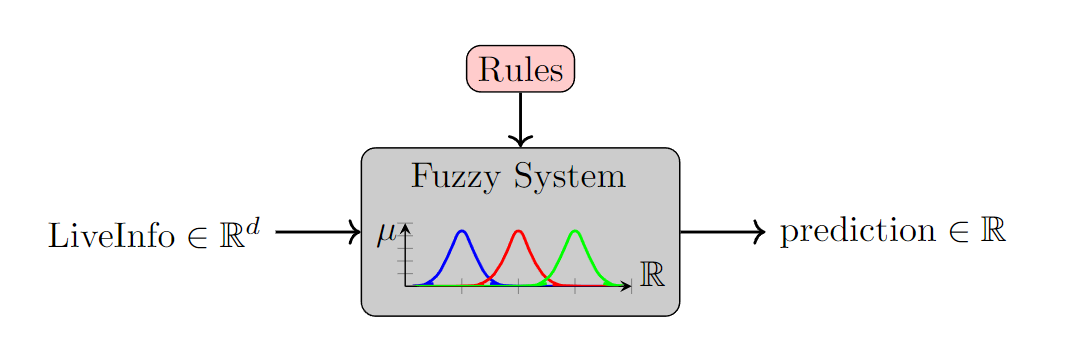
\includegraphics[width=0.9\textwidth]{figures/single-fuzzy-system.png}
	\end{figure}
\end{frame}



\begin{frame}
	\frametitle{Approach 1: Component Tuning}
	\begin{itemize}
		\item Explicit Fuzzy System for each tunable parameter
		      \begin{itemize}
			      \item Continuous representation of the parameter values
		      \end{itemize}
	\end{itemize}
	
	\begin{figure}
		\centering
		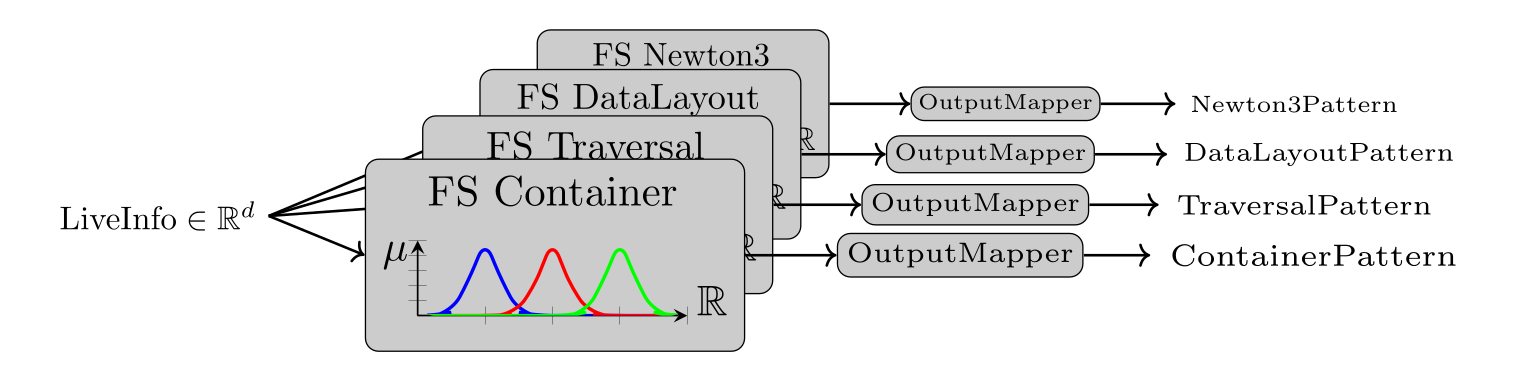
\includegraphics[width=1\textwidth]{figures/component-approach.png}
	\end{figure}
	
	\begin{itemize}
		{\small
		\item Example: \textbf{IF} avgParticlesPerCell is \textit{low} \textbf{AND} threadCount is \textit{low}\\ \qquad  \qquad \qquad  \textbf{THEN} traversal is \textit{vcl\_c06}
		      }
	\end{itemize}
	
	
\end{frame}


\begin{frame}
	\frametitle{Approach 2: Suitability Tuning}
	\begin{itemize}
		\item A Fuzzy System for \textbf{each} possible configuration
		\item Predict $suitability$ of each configuration
	\end{itemize}
	
	\begin{figure}
		\centering
		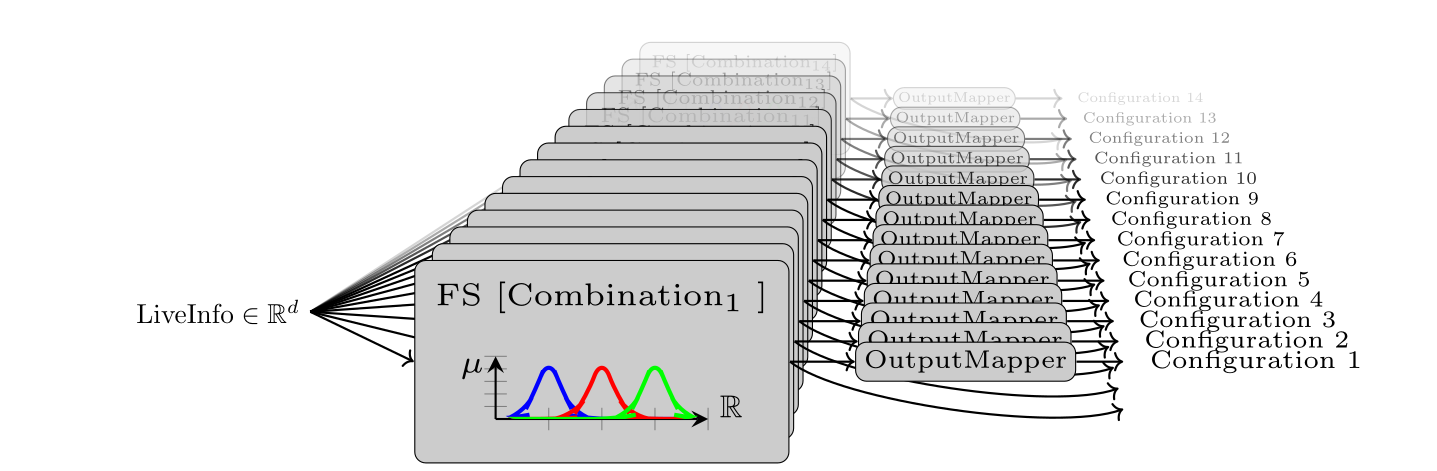
\includegraphics[width=1\textwidth]{figures/suitability-approach.png}
	\end{figure}
	
	\begin{itemize}
		{\small
		\item Example: \textbf{IF} threadCount is \textit{high} \textbf{AND} avgParticlesPerCell is \textit{low}\\ \qquad  \qquad \qquad \textbf{THEN} suitability\_LinkedCells\_AoS\_lc\_c18\_disabled is \textit{bad}
		      }
	\end{itemize}
	
\end{frame}


\begin{frame}
	\frametitle{Challenge 2: Expert Knowledge}
	
	\begin{itemize}
		\item How to design the Fuzzy System?
		      \begin{itemize}
			      \item Creating it manually?\\
			            \quad \xmark \; Requires extensive expert knowledge\\
			            \quad \xmark \; Difficult to formalize non-trivial knowledge
			      \item Extracting rules from data?\\
			            \quad \cmark \; No prior expert knowledge required\\
			            \quad \cmark \; Semi-automated process\\
		      \end{itemize}
	\end{itemize}
\end{frame}


\begin{frame}
	\frametitle{Data-Driven Rule Extraction}
	\begin{itemize}
		\item Machine learning to generate rules {\scriptsize  \cite{CROCKETT20062809}}
		      \begin{enumerate}
			      \item Train Decision Tree on the data
			      \item Decision Tree $\rightarrow$ Fuzzy Decision Tree
			      \item Fuzzy Decision Tree $\rightarrow$ Fuzzy Rules
		      \end{enumerate}
		\item Repeat to create overlapping rules (ensemble)
	\end{itemize}
\end{frame}

\begin{frame}
	\frametitle{Data $\rightarrow$ Decision Tree}
	
	\begin{itemize}
		\item Separate classes recursively with axis-aligned splits
		\item Corresponds to nested \textit{if-then-else} rules
		\item Tree contains the entire expert knowledge
	\end{itemize}
	
	\vspace{0.2cm}
	
	\begin{figure}
		\centering
		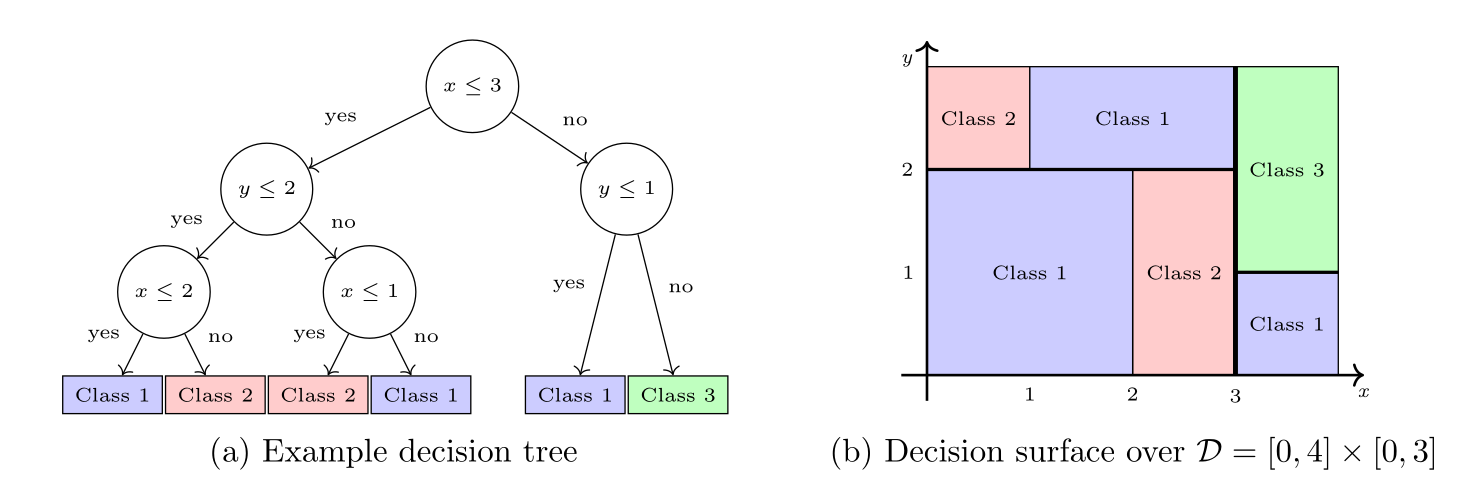
\includegraphics[width=1\textwidth]{figures/decision-tree.png}
	\end{figure}
	
\end{frame}

\begin{frame}
	\frametitle{Decision Trees $\rightarrow$ Fuzzy Decision Trees}
	
	\begin{itemize}
		\item Conversion: Each (crisp) split is turned into two fuzzy sets
		      \begin{itemize}
				\item Provides robustness against noise
				\item Both branches are considered
		      \end{itemize}
	\end{itemize}
	
	\begin{figure}
		\centering
		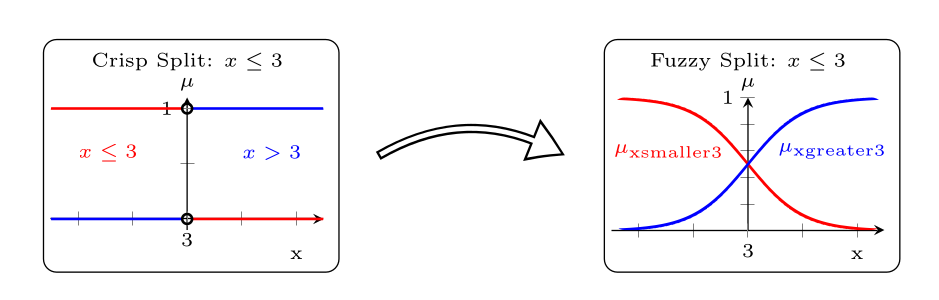
\includegraphics[width=8cm]{figures/leaf-conversion.png}
	\end{figure}
	
\end{frame}

\begin{frame}

	\begin{figure}
		\centering
		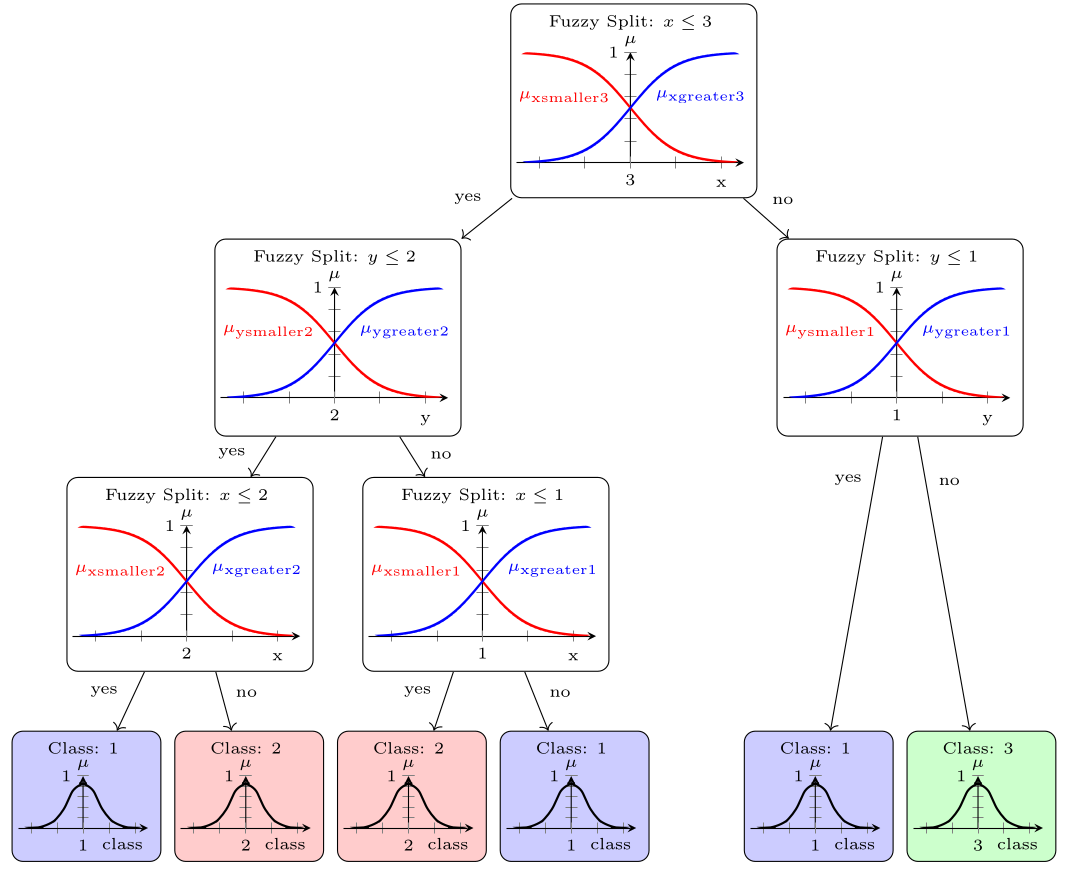
\includegraphics[width=0.9\textwidth]{figures/fuzzy-decision-tree.png}
	\end{figure}
	
\end{frame}

\begin{frame}

	\frametitle{Fuzzy Decision Trees $\rightarrow$ Fuzzy Rules}
	
	\begin{itemize}
		\item \textit{Unnest} the fuzzy decision tree
	\end{itemize}
	
	\begin{figure}
		\centering
		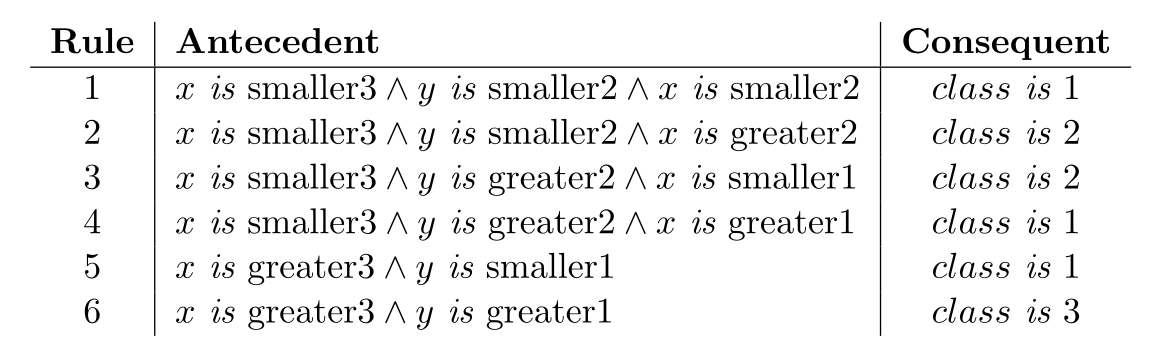
\includegraphics[width=0.9\textwidth]{figures/extracted-rules.png}
	\end{figure}
	
\end{frame}

\begin{frame}

	\frametitle{Decision Surfaces}
	
	\begin{figure}
		\begin{subfigure}[t]{0.49\textwidth}
			\centering
			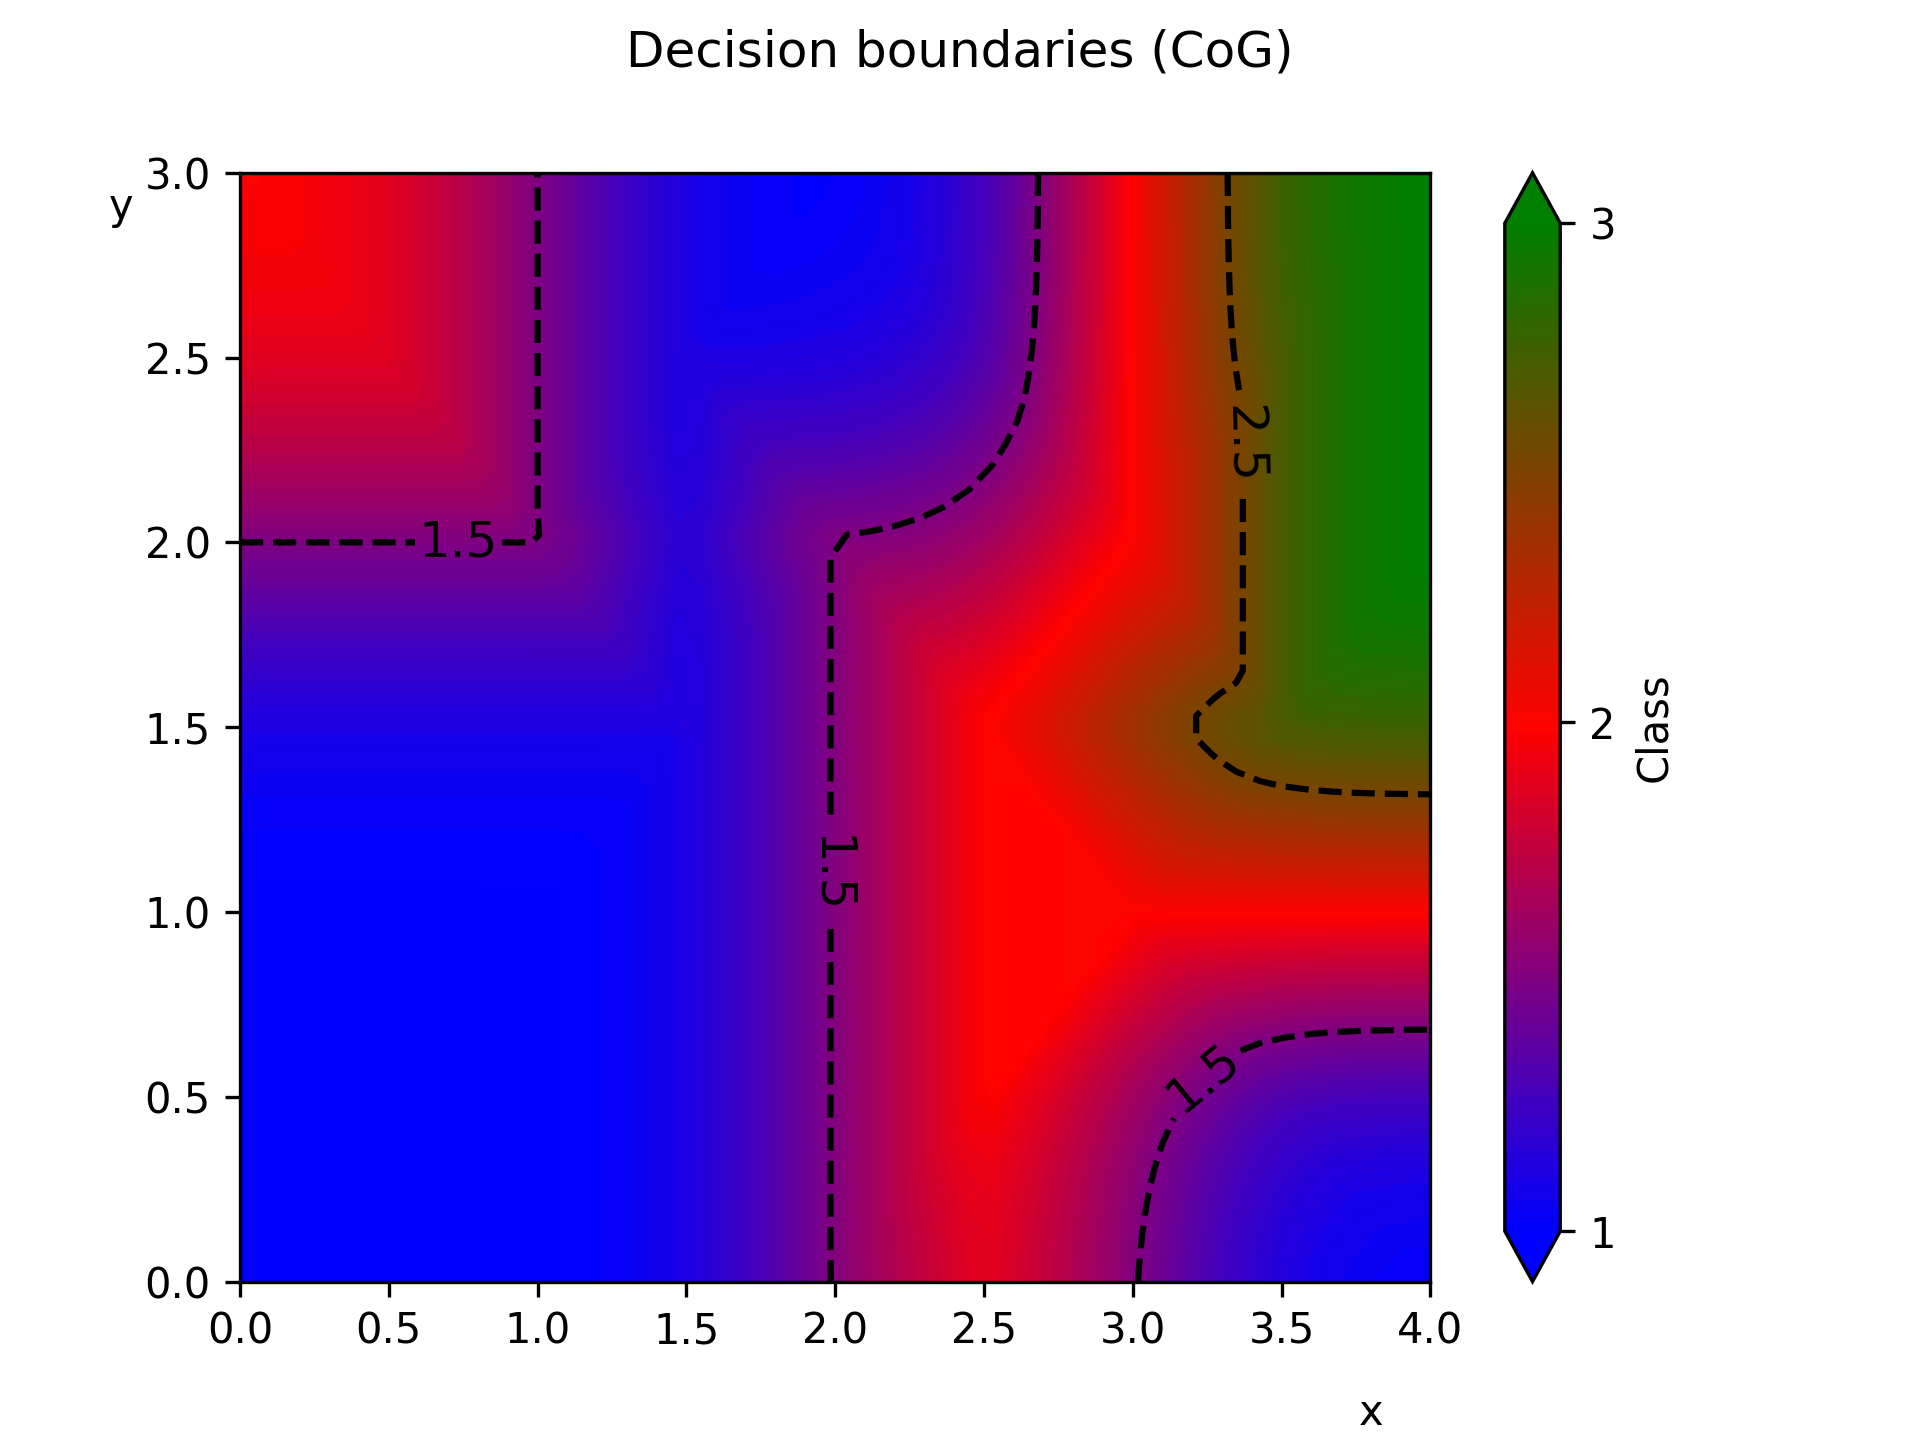
\includegraphics[width=1\textwidth, trim={0.5cm 0.5cm 1cm 1cm},clip]{figures/fuzzy_system_cog.png}
			\caption{Center of Gravity - Defuzzification}
		\end{subfigure}
		\begin{subfigure}[t]{0.49\textwidth}
			\centering
			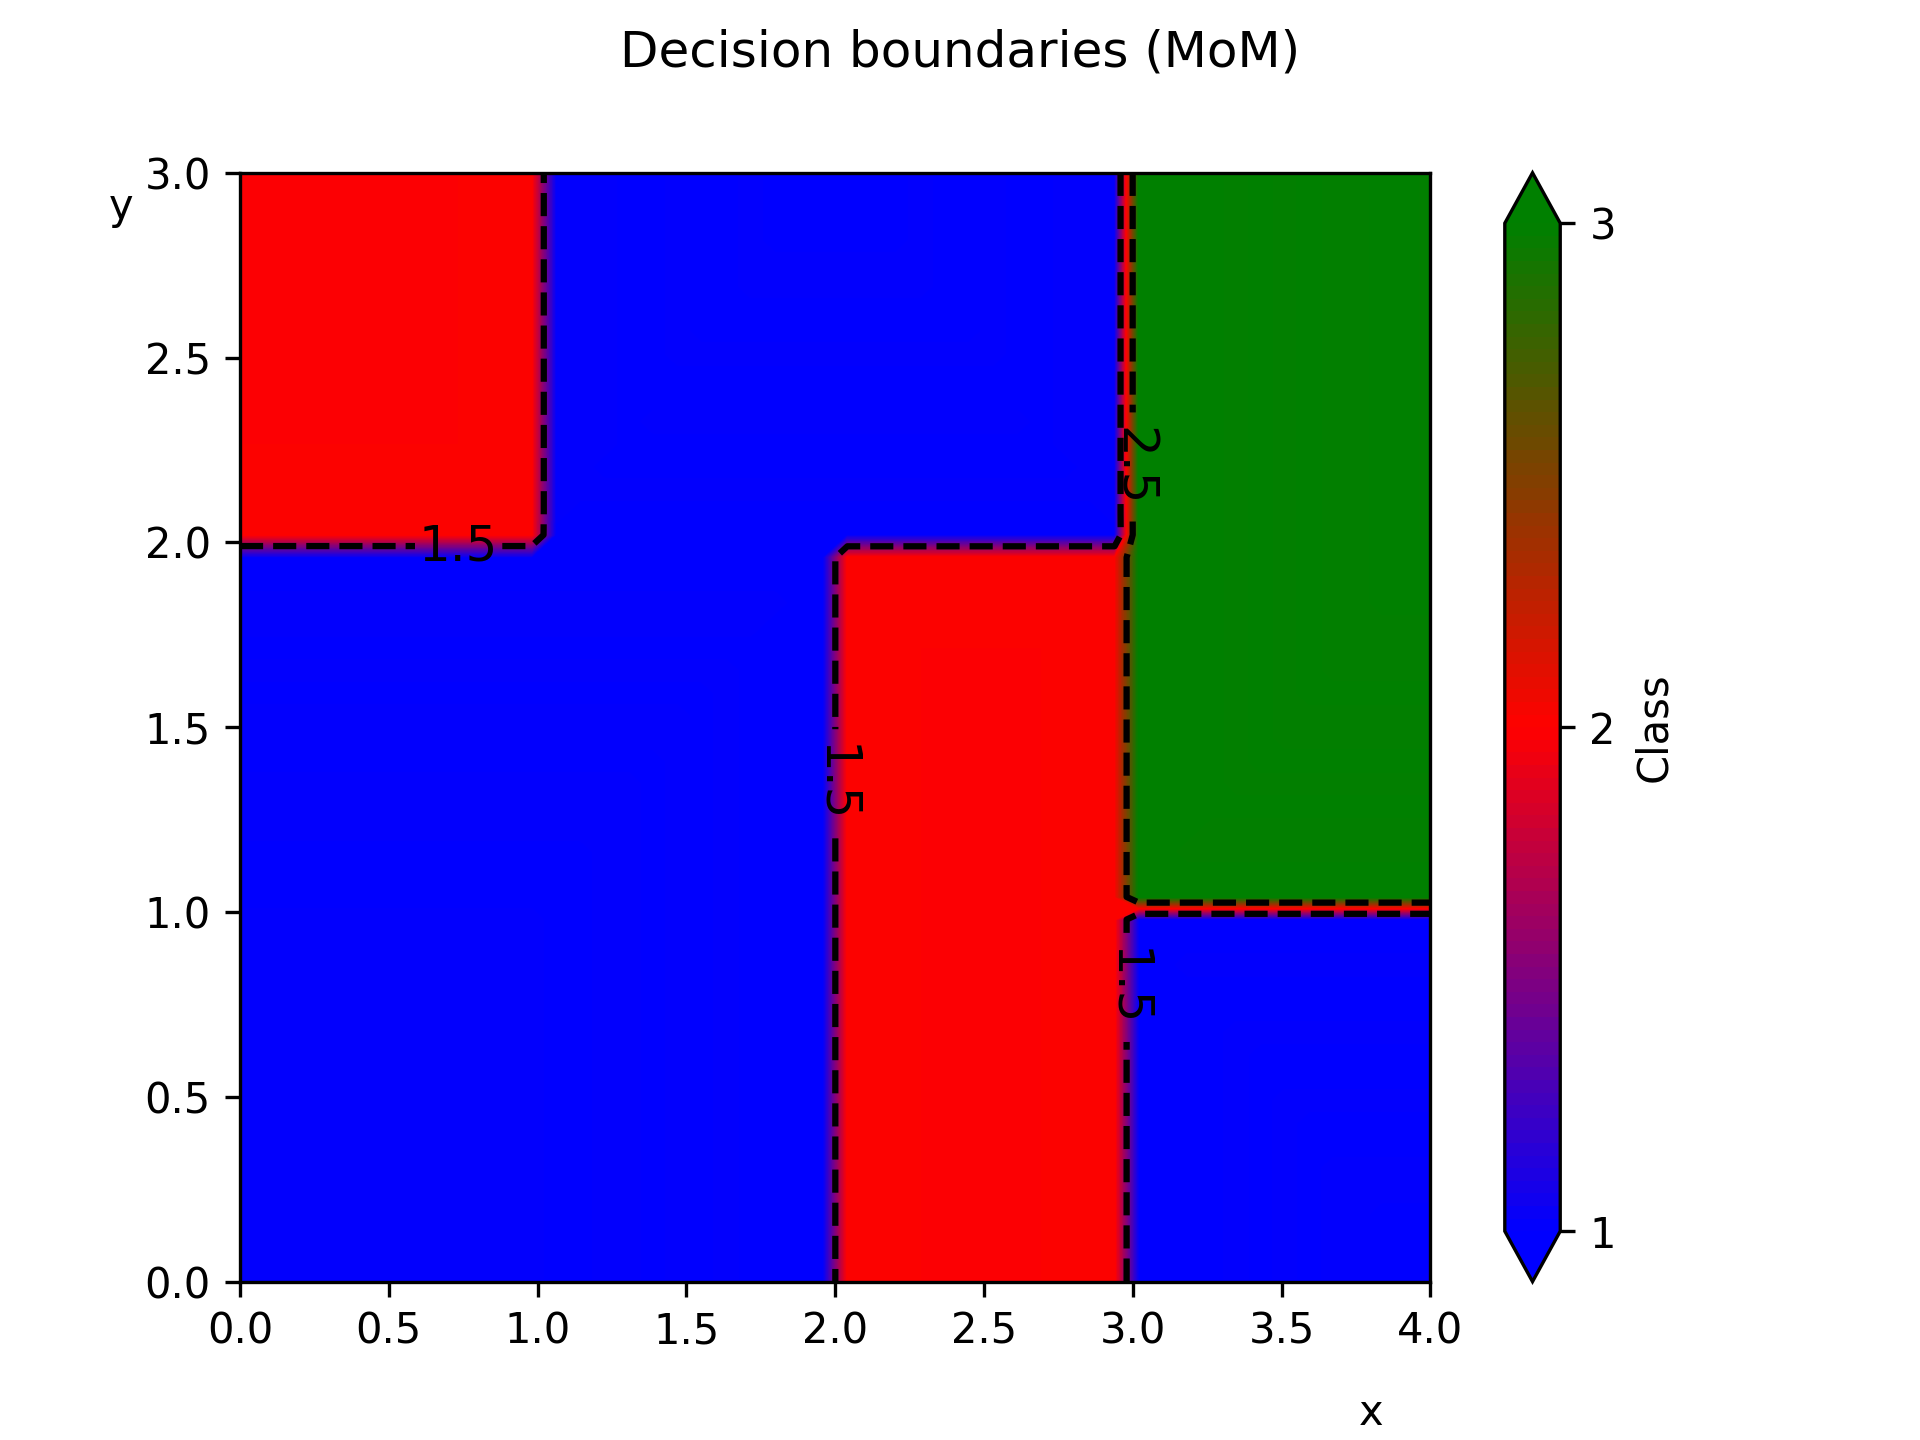
\includegraphics[width=1\textwidth, trim={0.5cm 0.5cm 1cm 1cm},clip]{figures/fuzzy_system_mom.png}
			\caption{Mean of Maxima - Defuzzification}
		\end{subfigure}
		\caption{Decision Surfaces of Fuzzy System}
	\end{figure}
	
\end{frame}


\begin{frame}
	\frametitle{Fuzzy Rule Extraction for \texttt{md\_flexible}}
	
	\begin{itemize}
		\item Collect dataset of \texttt{md\_flexible} simulations
		\item For each tuning phase $i$, store:
		      \begin{itemize}
			      \item LiveInfoData: {\footnotesize \texttt{maxDensity, homogeneity, threadCount, \dots} }
			      \item TuningData: {\footnotesize \texttt{Container, Traversal, Newton3, \dots, \textbf{Time}} }
		      \end{itemize}
		\item Introduce \textit{relative speed} metric
		      \begin{itemize}
			      \item Absolute time is not meaningful
			            \[ \text{relative speed}_{config}^{(i)} = \frac{\text{t}_{best}^{(i)}}{\text{t}_{\text{config}}^{(i)}} \]
		      \end{itemize}
	\end{itemize}
	
\end{frame}

\begin{frame}
	\frametitle{Resulting Dataset}
	
	\begin{itemize}
		\item Contains expected \textit{relative speed} based on:
		      \begin{itemize}
			      \item Simulation state
			      \item Configuration
		      \end{itemize}
	\end{itemize}
	
	\begin{figure}
		\centering
		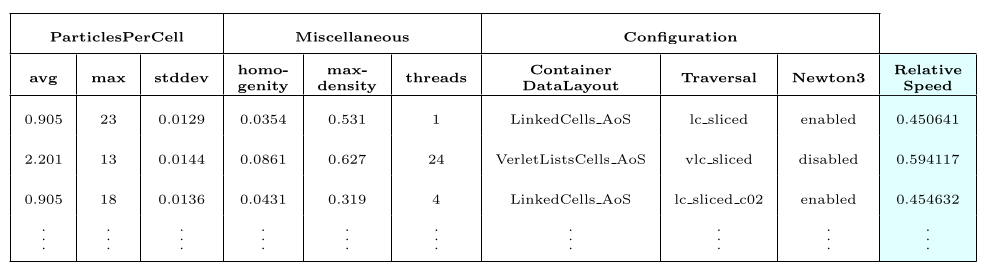
\includegraphics[width=1\textwidth]{figures/relative-speed-table.png}
	\end{figure}
	
\end{frame}

\begin{frame}
	\frametitle{Component Tuning - Rule Extraction}
	
	\begin{enumerate}
		\item Combine \textit{good} values for each simulation state
		\item Extract rules for each parameter
	\end{enumerate}
	
	\begin{figure}
		\centering
		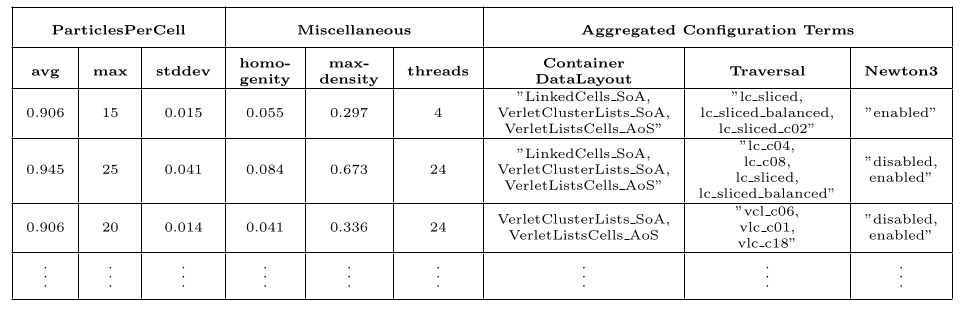
\includegraphics[width=0.93\textwidth, trim={0 3.8cm 0 0},clip]{figures/aggregated-data-component.png}
		\vspace{1.5cm}
		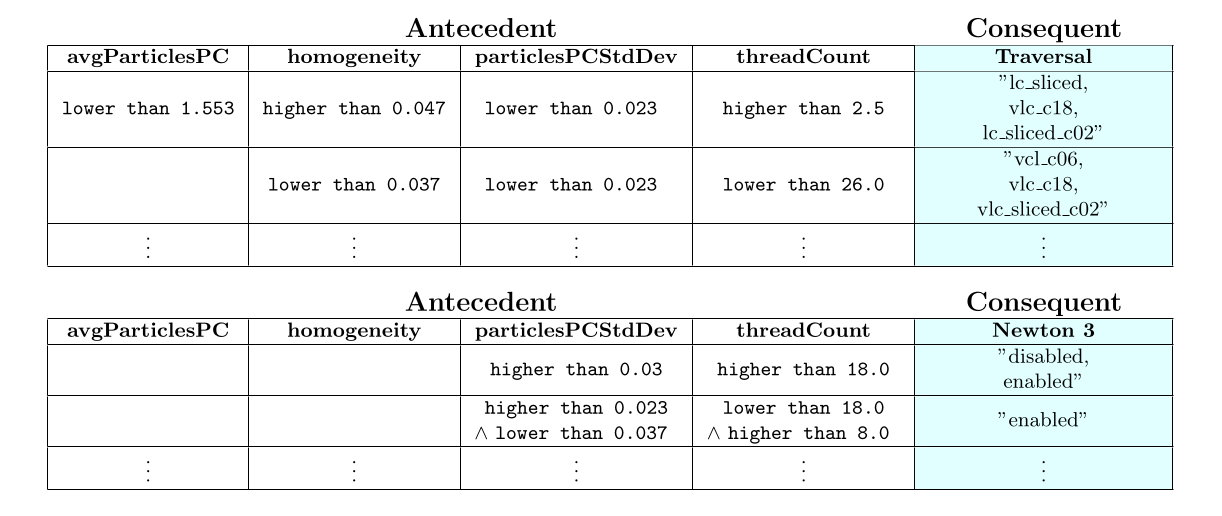
\includegraphics[width=0.98\textwidth, trim={0 8cm 0 0},clip]{figures/final-rules-component.png}
	\end{figure}
\end{frame}

\begin{frame}
	\frametitle{Suitability Tuning - Rule Extraction}
	
	\begin{enumerate}
		\item Assign suitability classes to each entry in the dataset
		\item Group dataset by configuration
		\item Rule Extraction for each configuration
	\end{enumerate}
	
	
	\begin{figure}
		\centering
		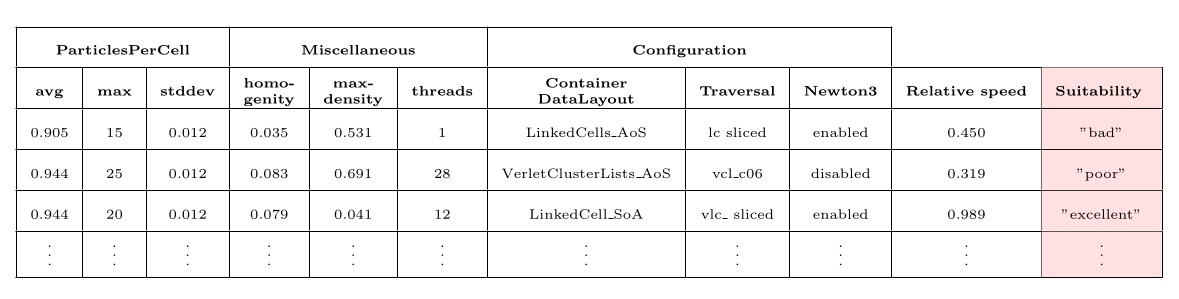
\includegraphics[width=1\textwidth, trim={0 2.25cm 0 0},clip]{figures/aggregated-data-suitability.png}
		\vspace{1.5cm}
		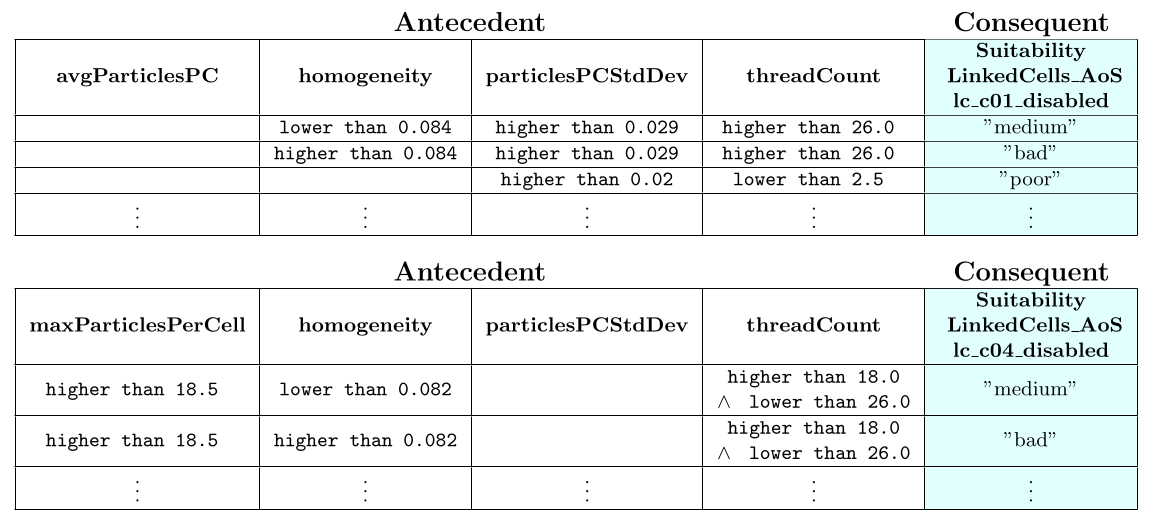
\includegraphics[width=1\textwidth, trim={0 9cm 0 0.1cm},clip]{figures/final-rules-suitability.png}
	\end{figure}
\end{frame}

\section{Benchmarks}
\begin{frame}
	\frametitle{Benchmark 1: Exploding Liquid}
	\begin{itemize}
		\item Fuzzy Tuning Approaches:
		      \begin{itemize}
			      {\footnotesize
			      \item Very short tuning phases
			      \item Selected configurations perform well
			      \item Winning configurations are (mostly) equivalent
			            }
		      \end{itemize}
	\end{itemize}
	
	\begin{figure}
		\centering
		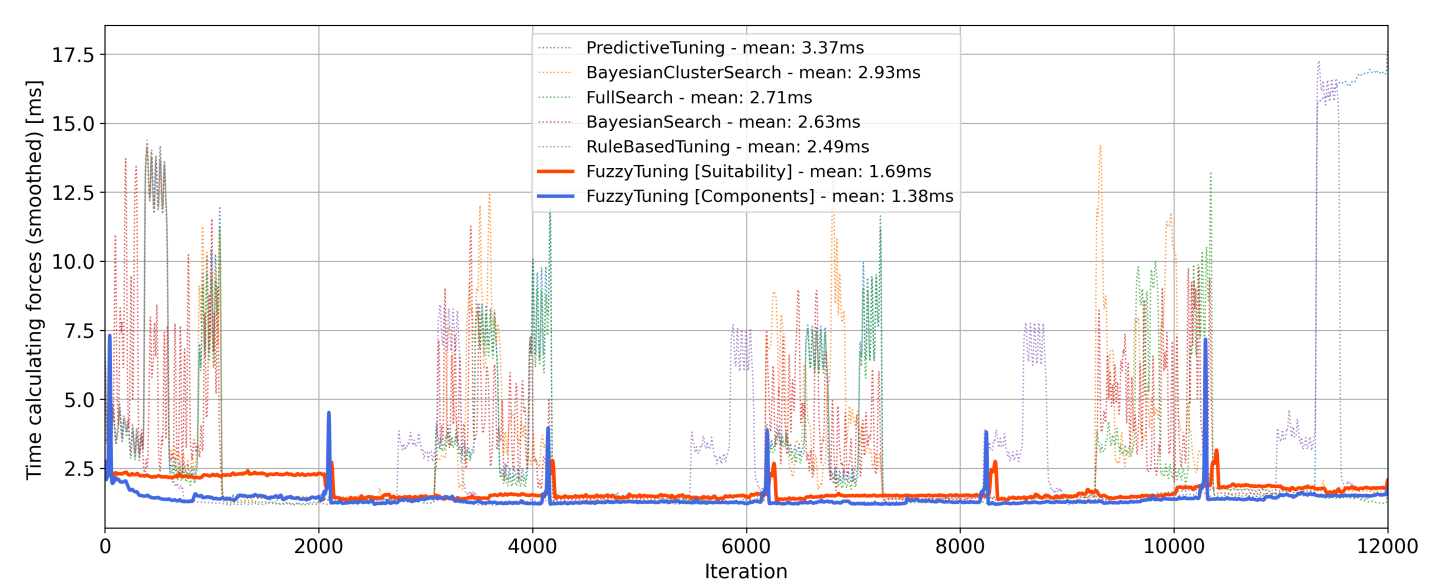
\includegraphics[width=1\textwidth]{figures/exploding-liquid-timings.png}
	\end{figure}
\end{frame}

\begin{frame}
	\frametitle{Total Time: Exploding Liquid}
	\begin{itemize}
		\item Fuzzy Tuning is good because:
		      \begin{itemize}
			      \item Few evaluated configurations
			      \item Good evaluated configurations
		      \end{itemize}
		\item Massive reduction in time spent tuning
		      \begin{itemize}
			      \item[$\rightarrow$] More frequent tuning phases
		      \end{itemize}
	\end{itemize}
	
	\begin{figure}
		\centering
		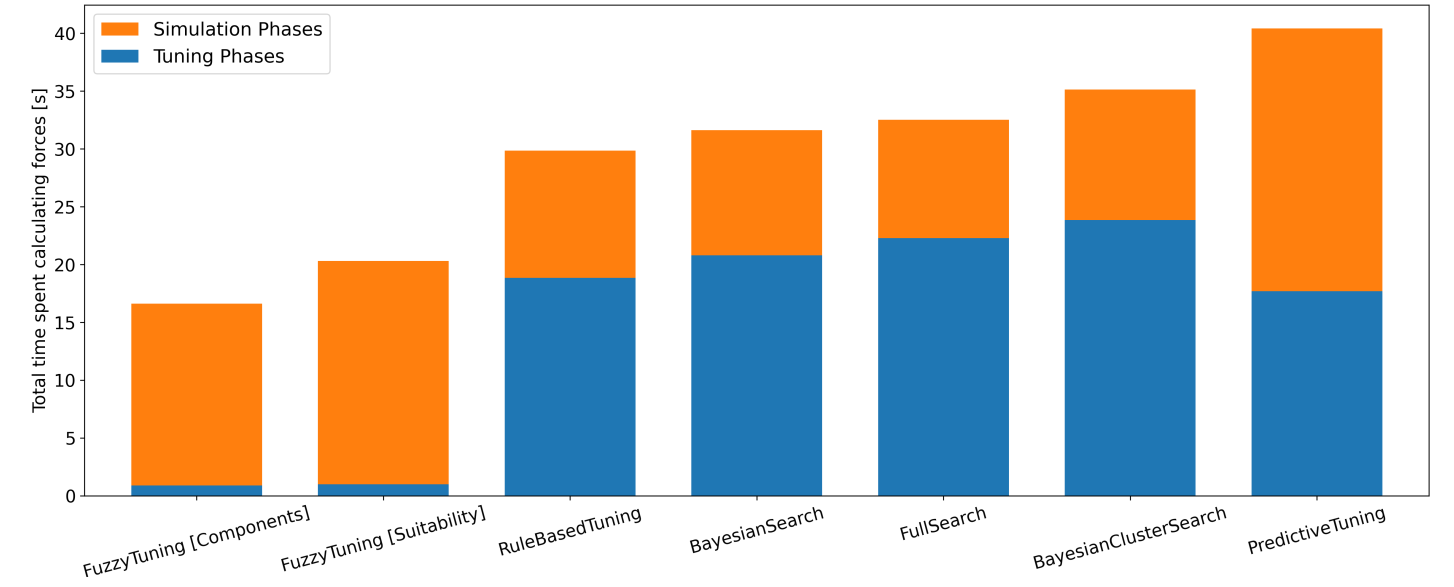
\includegraphics[width=0.95\textwidth]{figures/exploding-liquid-total.png}
	\end{figure}
\end{frame}

\begin{frame}
	\frametitle{Benchmark 2: Spinodal Decomposition (MPI)}
	
	\begin{itemize}
		\item Component approach performs well
		\item Suitability approach misses the optimal configuration
		      \begin{itemize}
			      \item However: no tuning overhead
			      \item Can this make up for the suboptimal configurations?
		      \end{itemize}
	\end{itemize}
	
	\vspace{-0.1cm}
	
	\begin{figure}
		\centering
		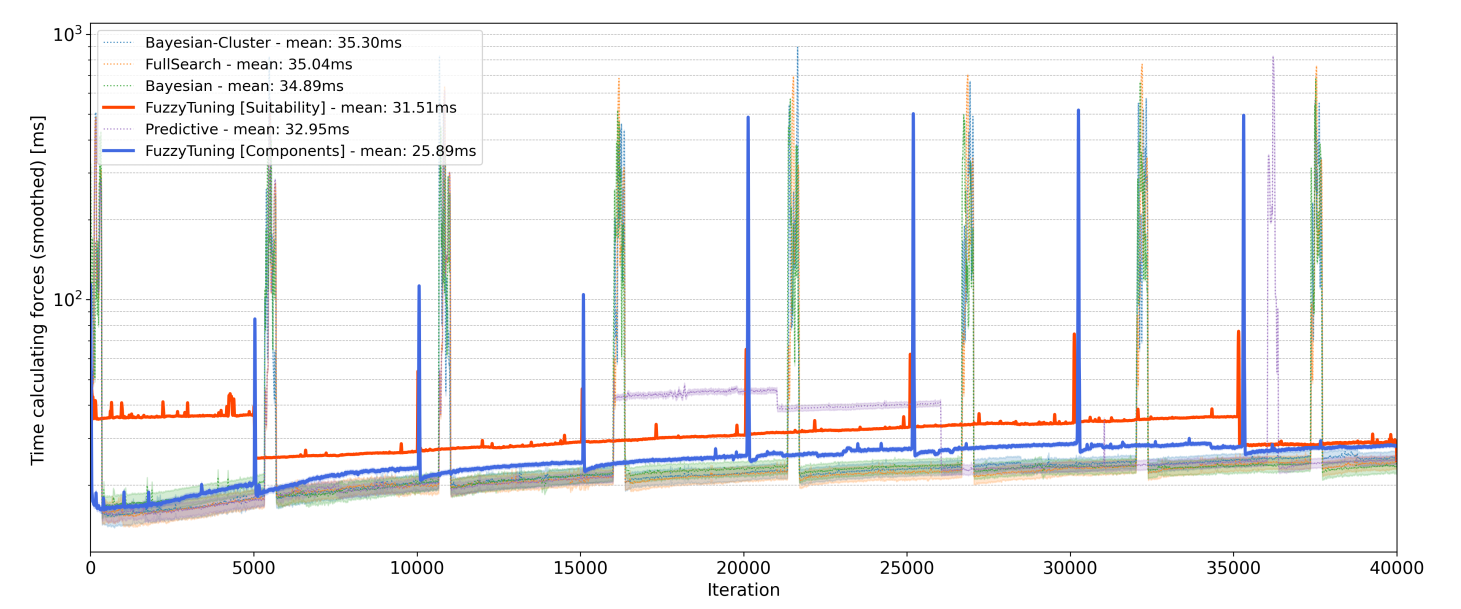
\includegraphics[width=1\textwidth]{figures/spinodal-timings.png}
	\end{figure}
\end{frame}

\begin{frame}
	\frametitle{Comparison and Evaluation: Spinodal Decomposition}
	
	\begin{itemize}
		\item Component tuning wins again
		\item Suitability tuning:
		      \begin{itemize}
			      \item Fast tuning phases compensate for suboptimal configurations!
			      \item Improvement: Encourage longer tuning phases
			            \begin{itemize}
				            \item Increase suitability threshold {\scriptsize (Top 10\% $\rightarrow$ Top 30\%)}
			            \end{itemize}
		      \end{itemize}
	\end{itemize}
	
	\begin{figure}
		\centering
		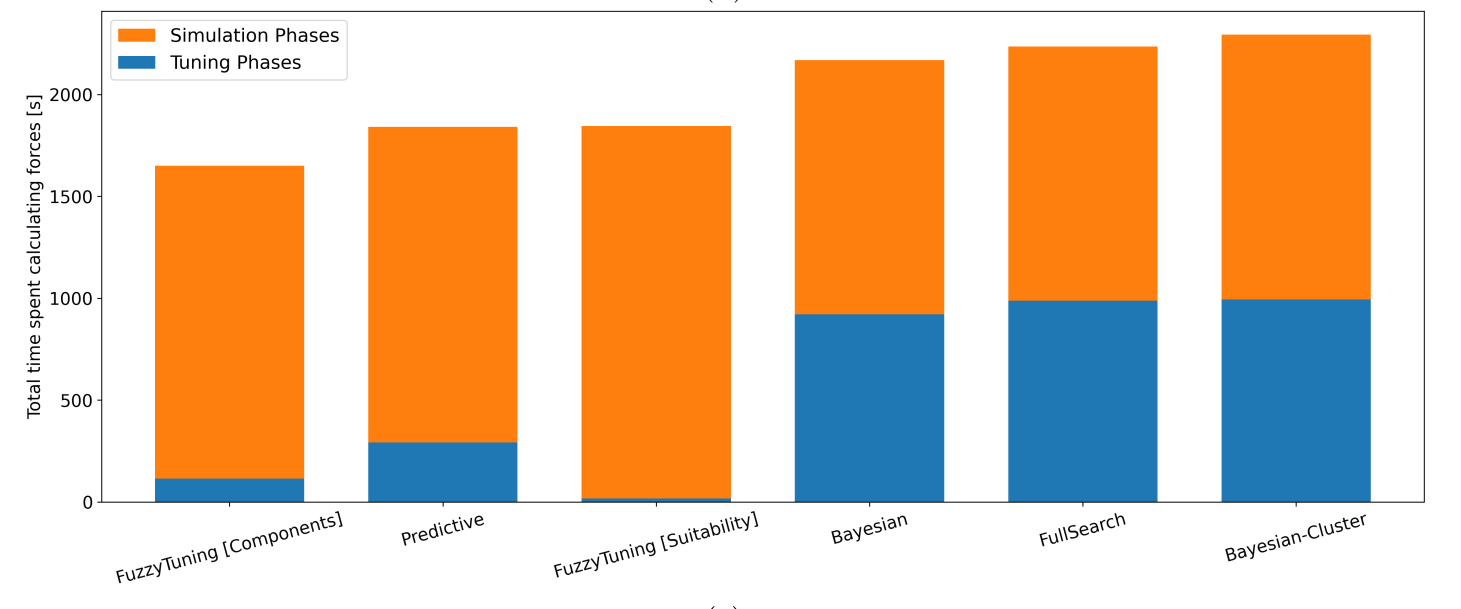
\includegraphics[width=0.92\textwidth]{figures/spinodal-total.png}
	\end{figure}
\end{frame}


\section{Conclusion}

\begin{frame}
	\frametitle{Conclusion}
	\begin{itemize}
		\item Fuzzy Tuning is very promising for AutoPas
		      \begin{itemize}
			      \item Massive reduction in tuning overhead
			      \item Reduction of total simulation time (up to factor 1.96x)
			      \item Among the best tuning strategies (but very complex)
		      \end{itemize}
		      \pause
		\item Ongoing Challenge:
		      \begin{itemize}
			      \item Rule generation \\
			            \quad \xmark \; Requires a lot of data (1.1GB) \\
			            \quad \xmark \; Unappealing for users \\
			            \quad \xmark \; No universal solution (showed some generalization)
		      \end{itemize}
	\end{itemize}
\end{frame}


\begin{frame}
	\frametitle{Improvement Ideas}
	\begin{itemize}
		\item Dynamic Rule Generation
		      \begin{itemize}
			      \item Update expert knowledge on the fly
			      \item Automatically adapt to new scenarios
		      \end{itemize}
		\item Improvements to the Tuning Process
		      \begin{itemize}
			      \item Investigate \textit{early stopping} mechanism
			      \item Dismiss slow configurations early
			      \item Solve tuning overhead once and for all?
		      \end{itemize}
		\item Simplification of the Model
		      \begin{itemize}
			      \item Ensemble of Decision Trees instead of Fuzzy Systems
			      \item Maybe comparable results?
		      \end{itemize}
	\end{itemize}
\end{frame}


\begin{frame}
	\begin{center}
		\vspace{1cm}
		{\large \textbf{Thank you for your attention!}}
		
		\vspace{2cm}
		
		\Huge{Questions?}
	\end{center}
\end{frame}

\begin{frame}[allowframebreaks, noframenumbering]
	\frametitle{References}
	\footnotesize
	\bibliographystyle{apalike}
	\bibliography{literature}
\end{frame}

\appendix

\begin{frame}
	\frametitle{Backup: What happens on new scenarios?}
	
	\begin{itemize}
		\item Exploding Liquid: bigger $\varepsilon$ $\rightarrow$ more spacing
		\item Component Tuning is winning again
	\end{itemize}
	
	\begin{figure}
		\centering
		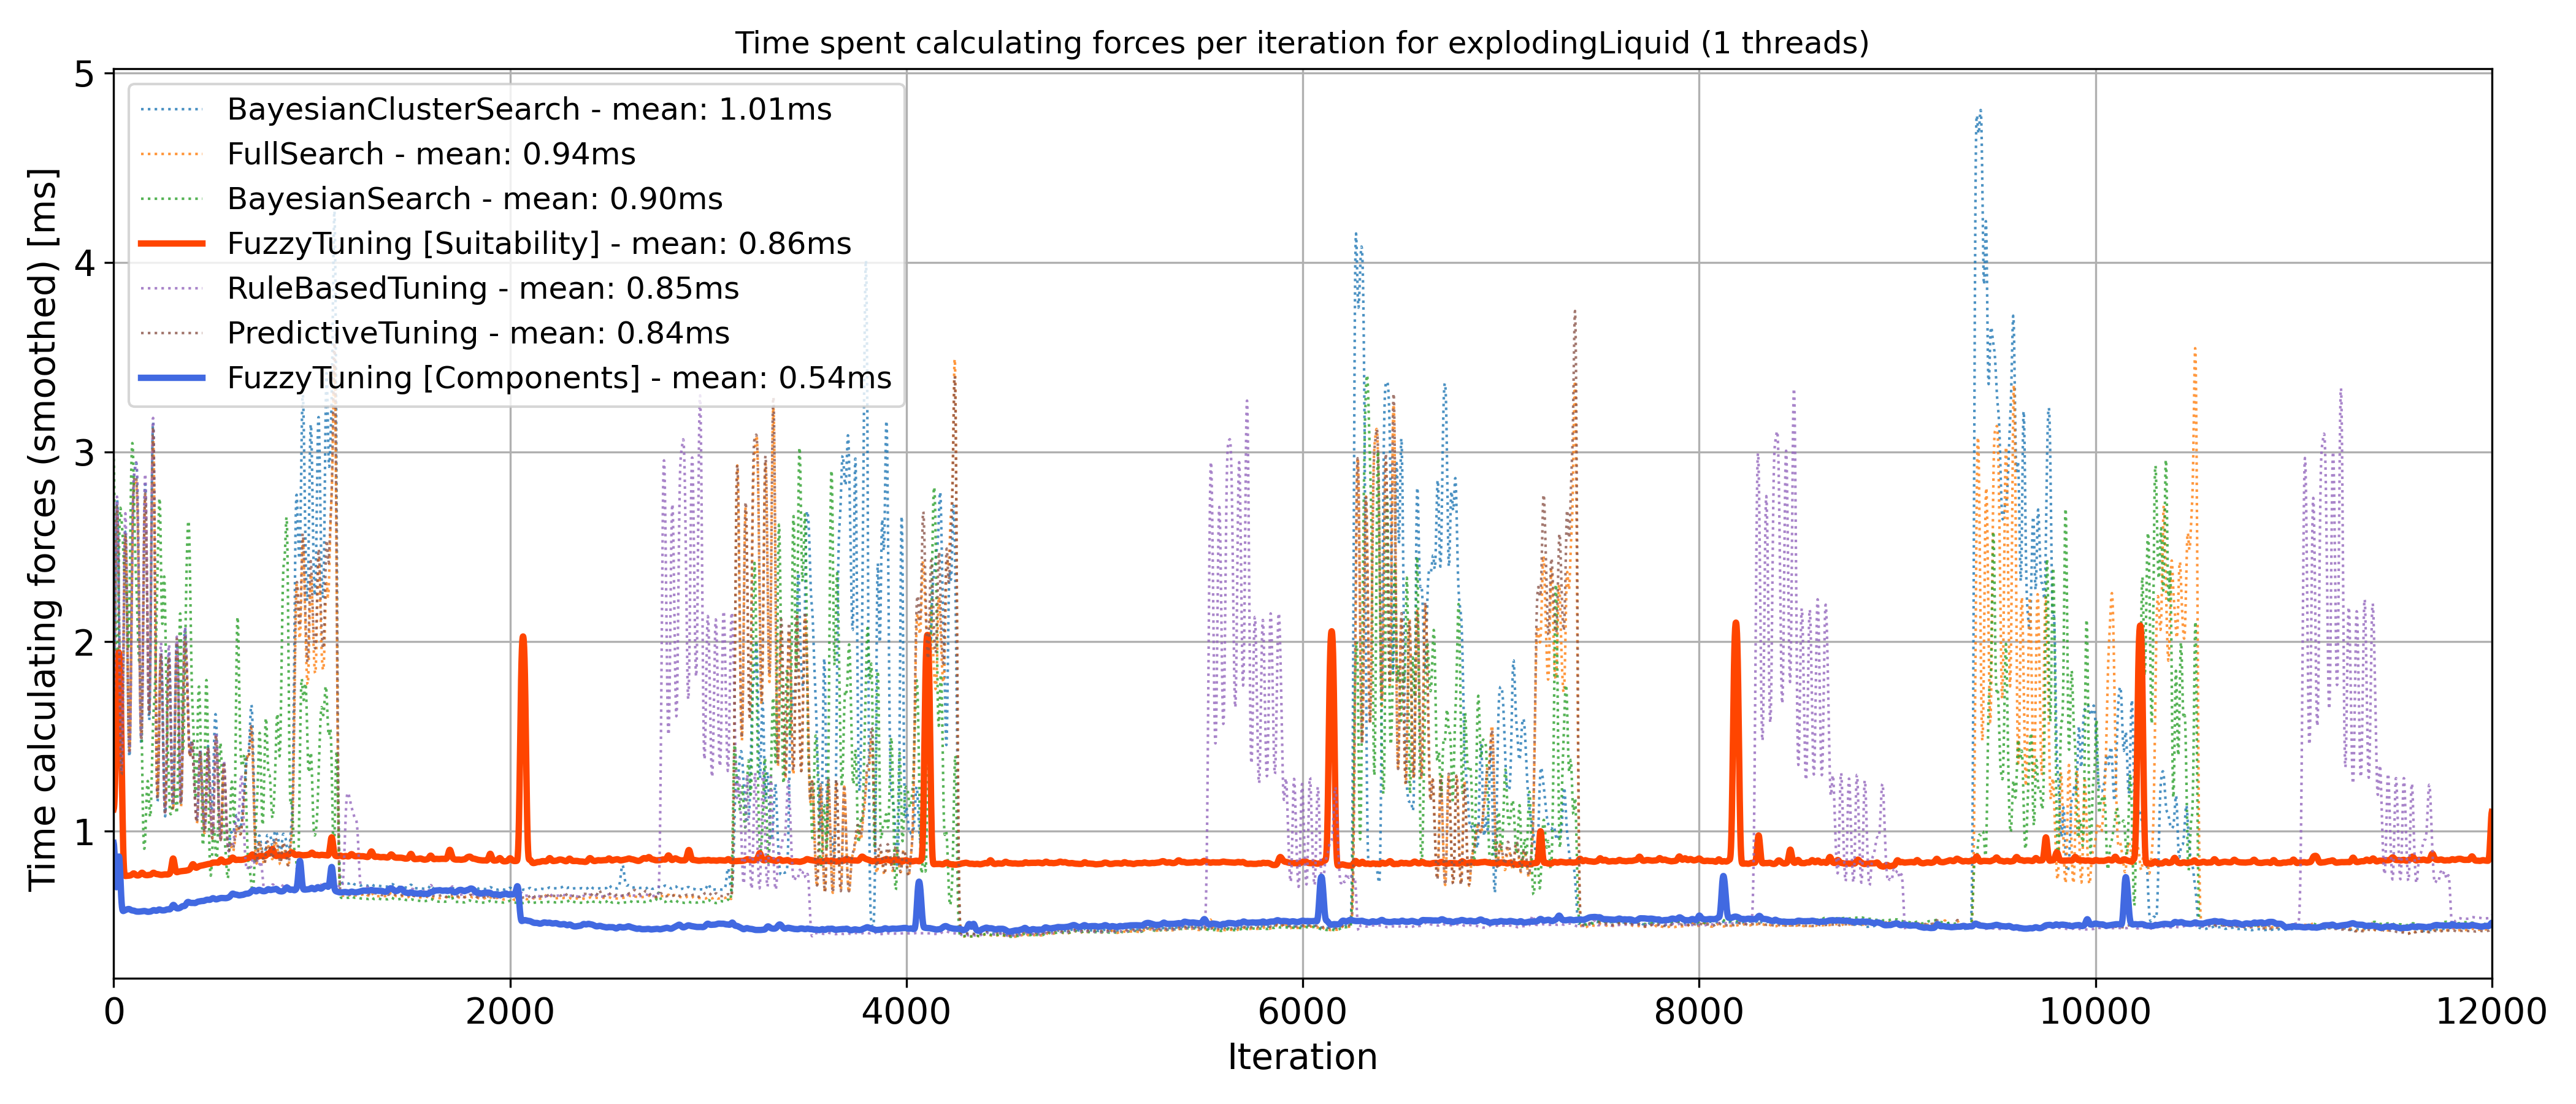
\includegraphics[width=1\textwidth]{figures/exploding-liquid-timings-eps.png}
	\end{figure}
\end{frame}

\begin{frame}
	\frametitle{Backup: Optimal Suitability Threshold}
	
	\begin{itemize}
		\item Goal: find optimal hyperparameters for suitability-approach
	\end{itemize}
	
	\begin{figure}
		\centering
		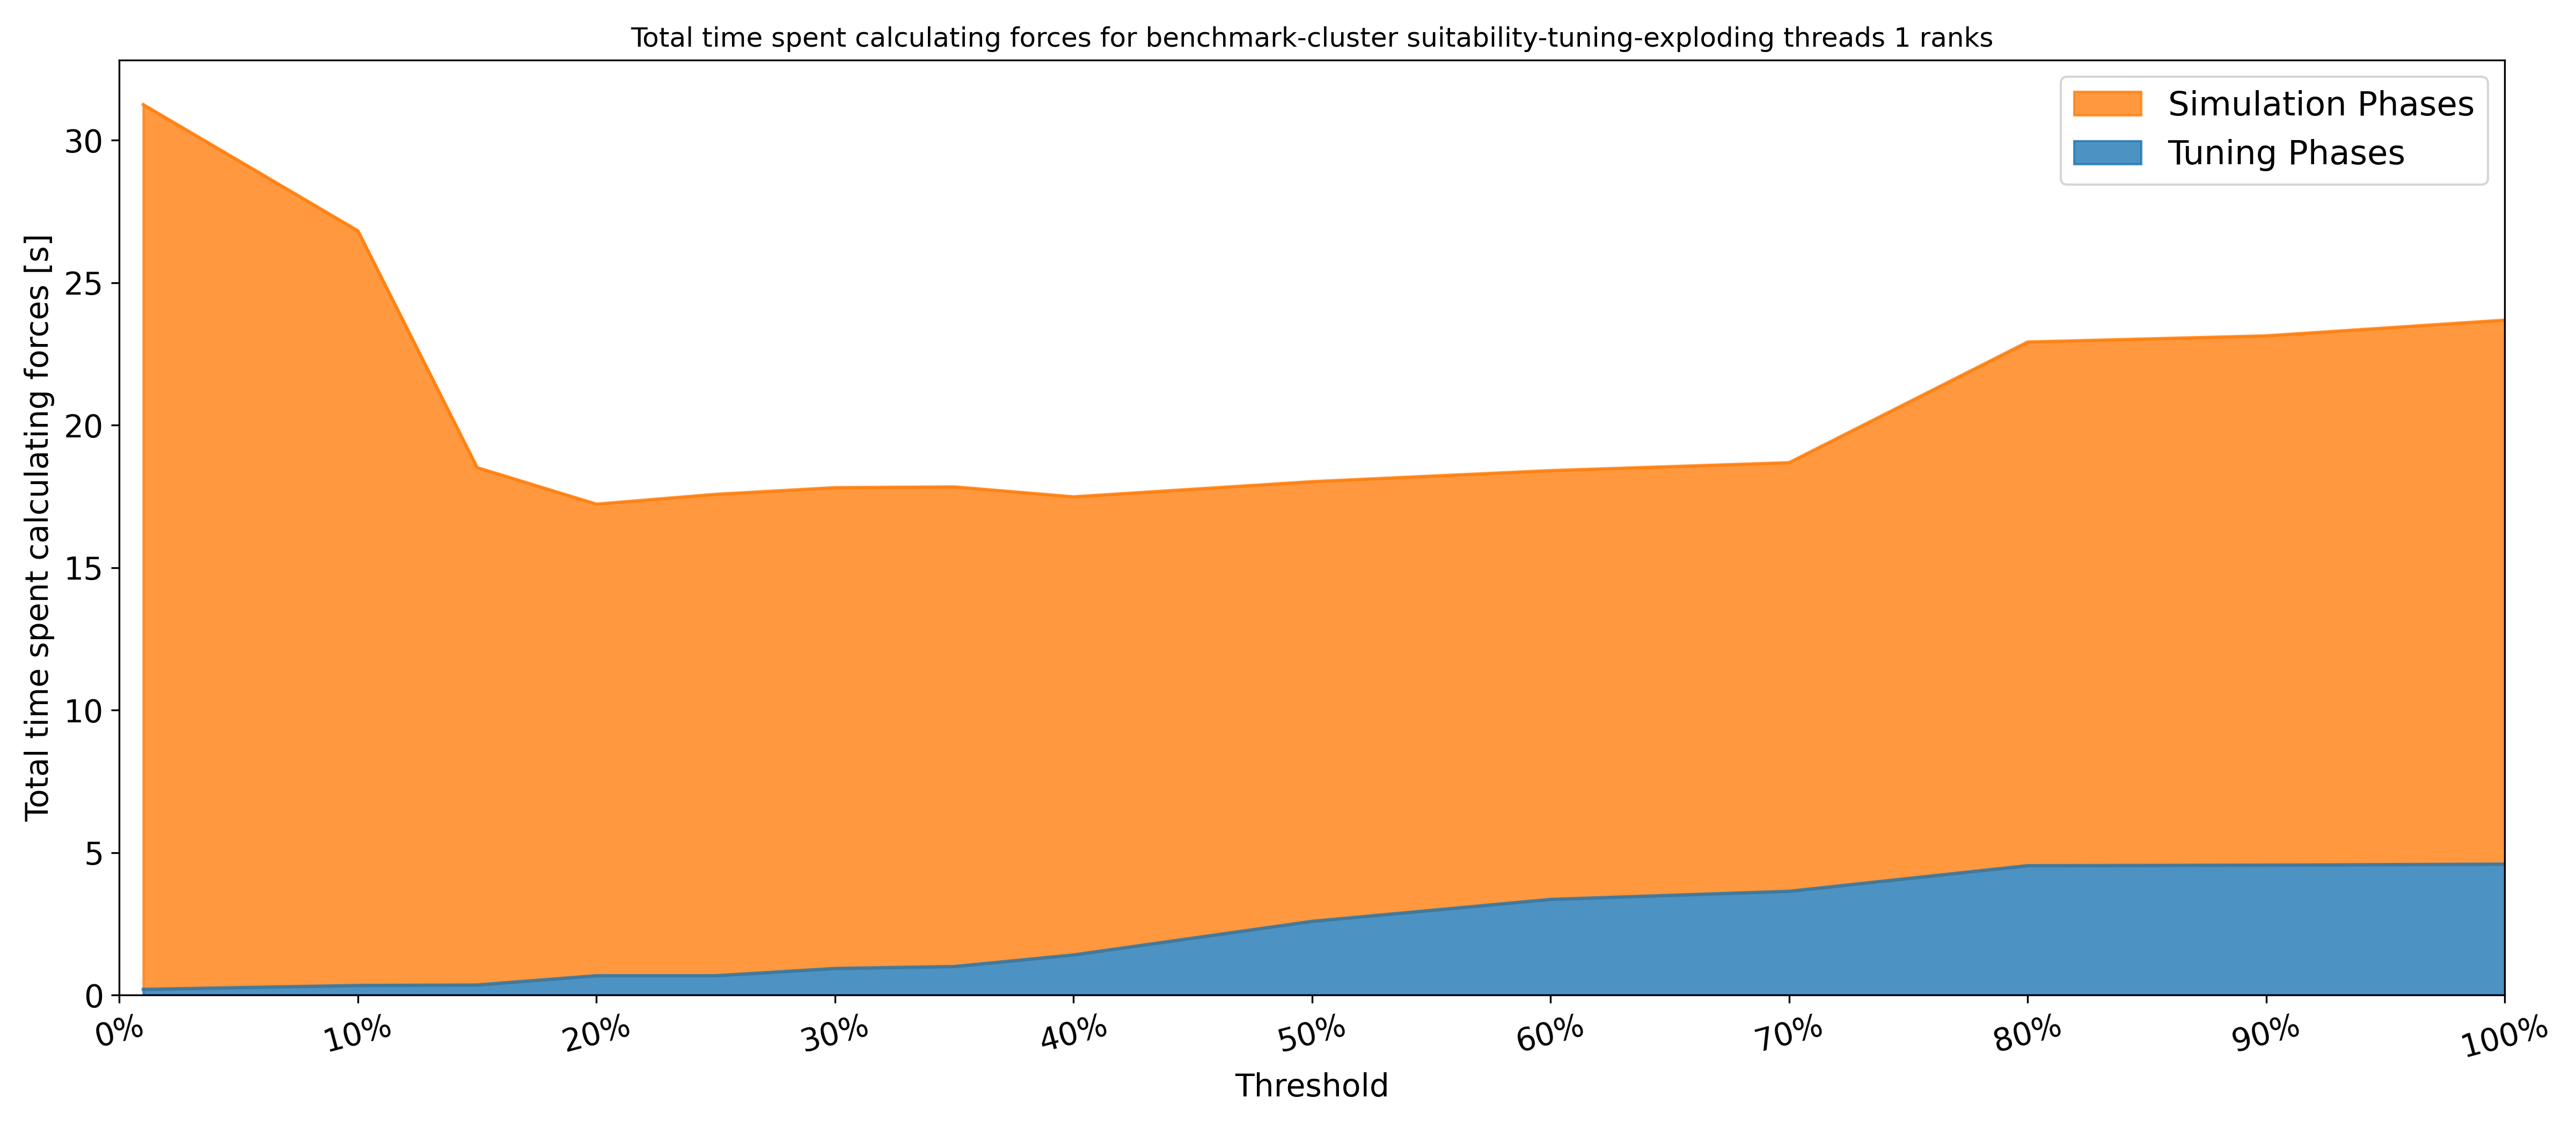
\includegraphics[width=1\textwidth]{figures/suitability-search.png}
	\end{figure}
\end{frame}

\begin{frame}
	\frametitle{Backup: Linguistic Variables for Component Tuning}
	
	\begin{figure}
		\centering
		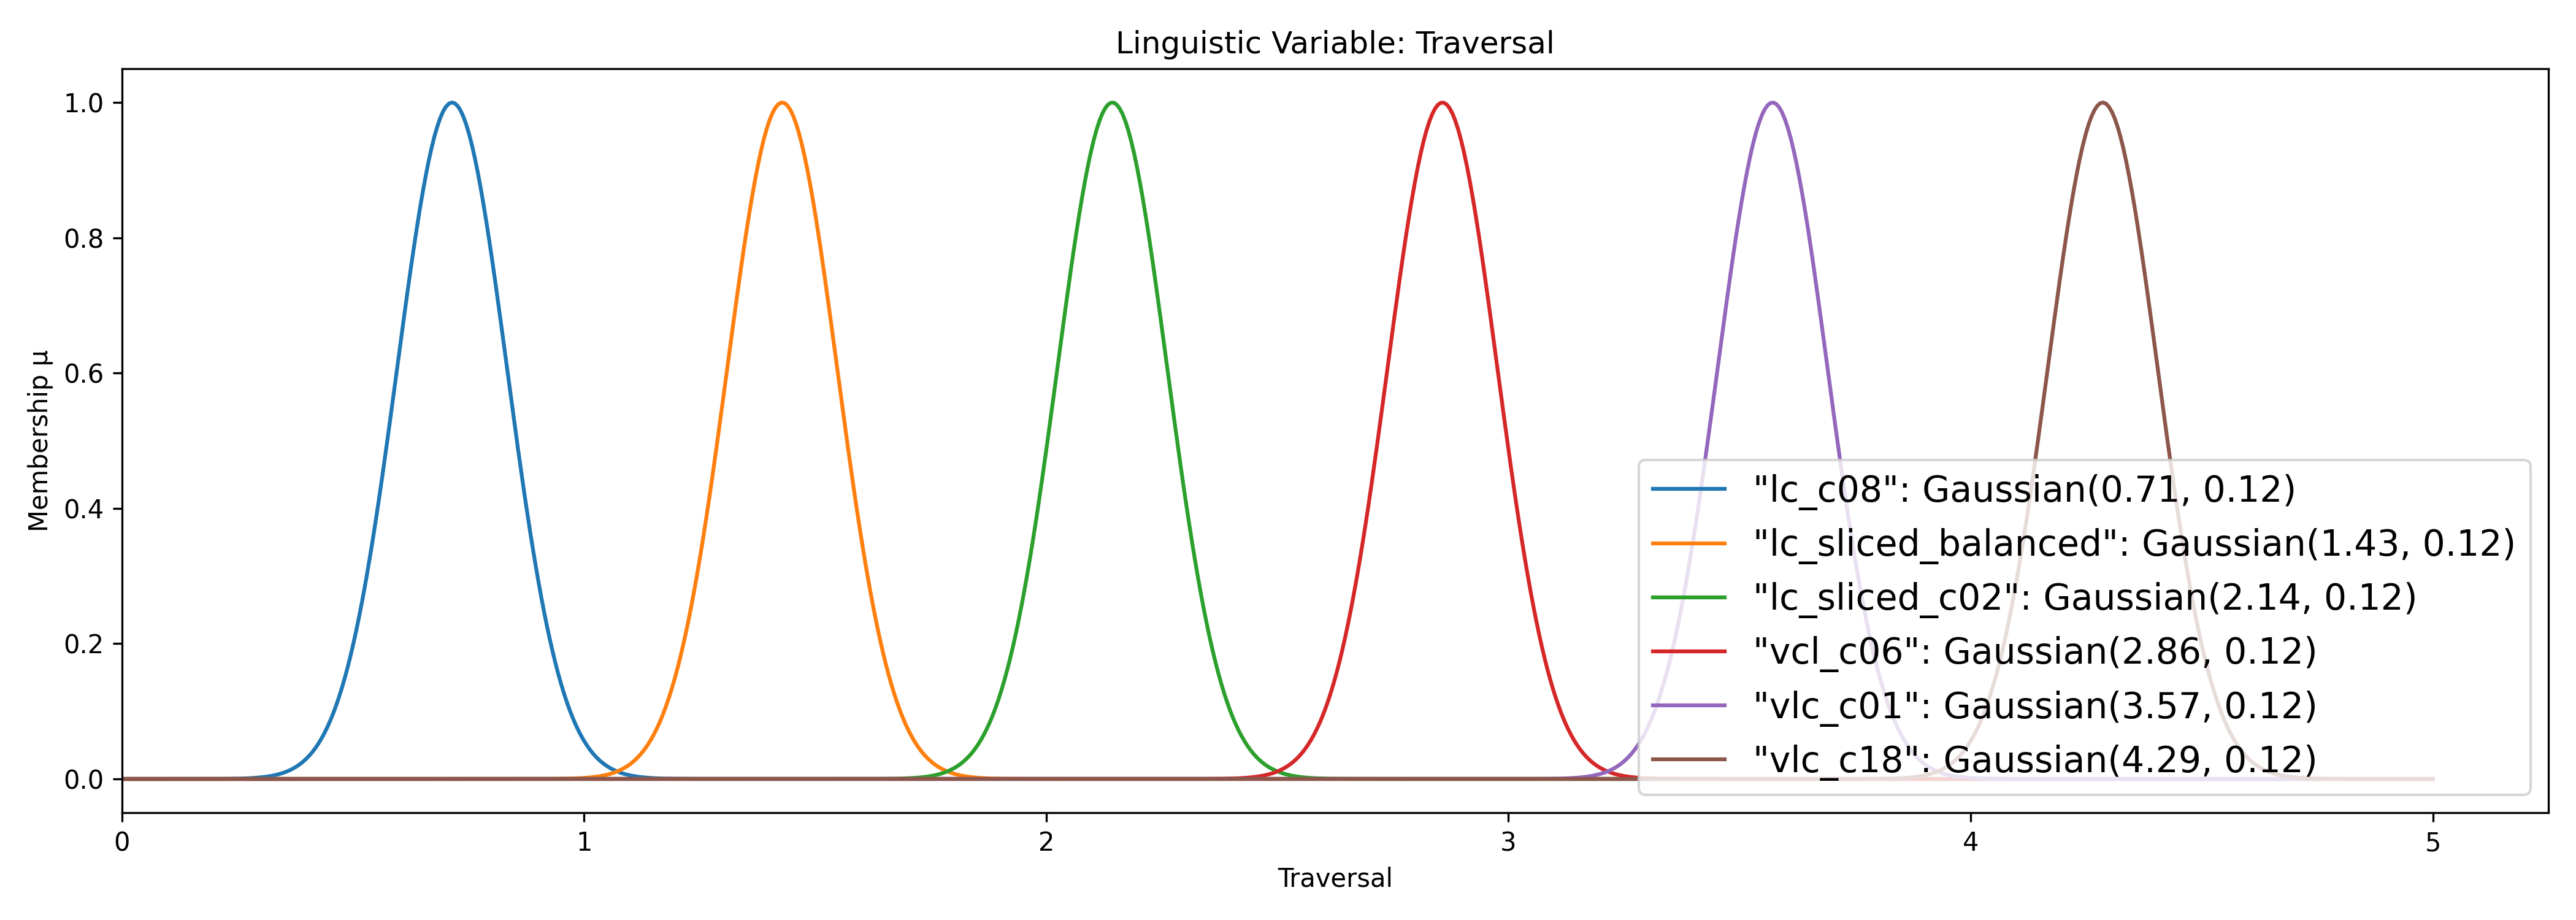
\includegraphics[width=1\textwidth]{figures/component-linguistic-variable.png}
	\end{figure}
	
\end{frame}

\begin{frame}
	\frametitle{Backup: Linguistic Variables for Suitability Tuning}
	\begin{figure}
		\centering
		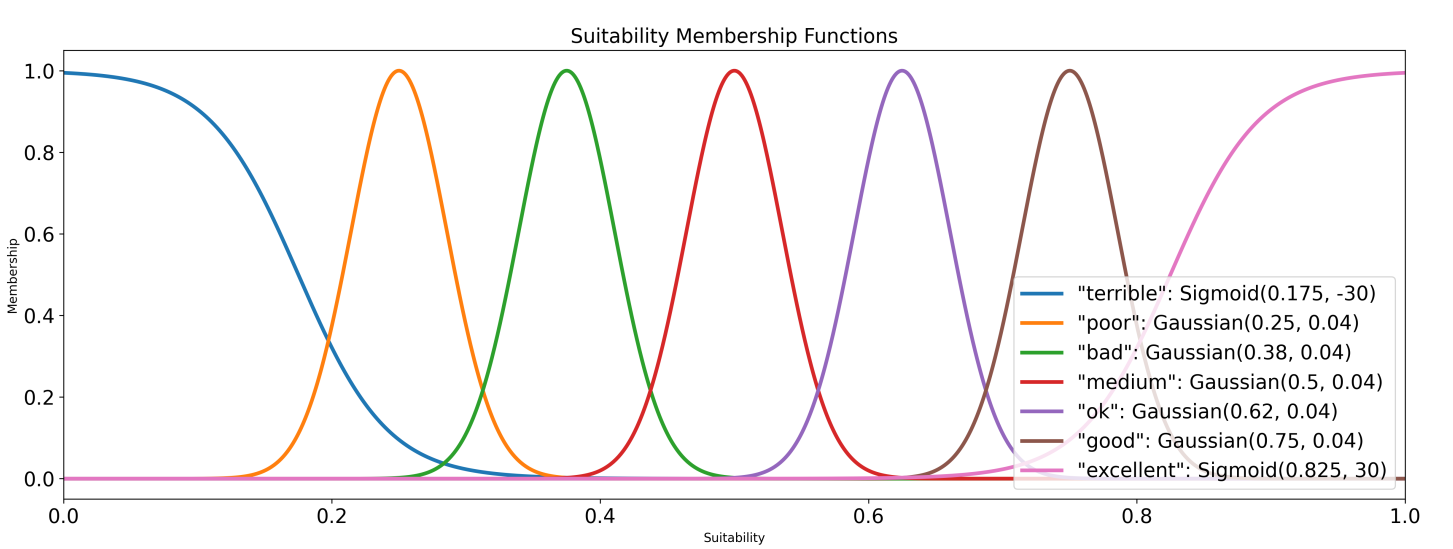
\includegraphics[width=1\textwidth]{figures/suitability-linguistic-variable.png}
	\end{figure}
	
\end{frame}


\begin{frame}
	\frametitle{Backup: Speedup Distribution}
	
	\begin{itemize}
		\item How good is the average configuration?
	\end{itemize}
	
	\begin{figure}
		\centering
		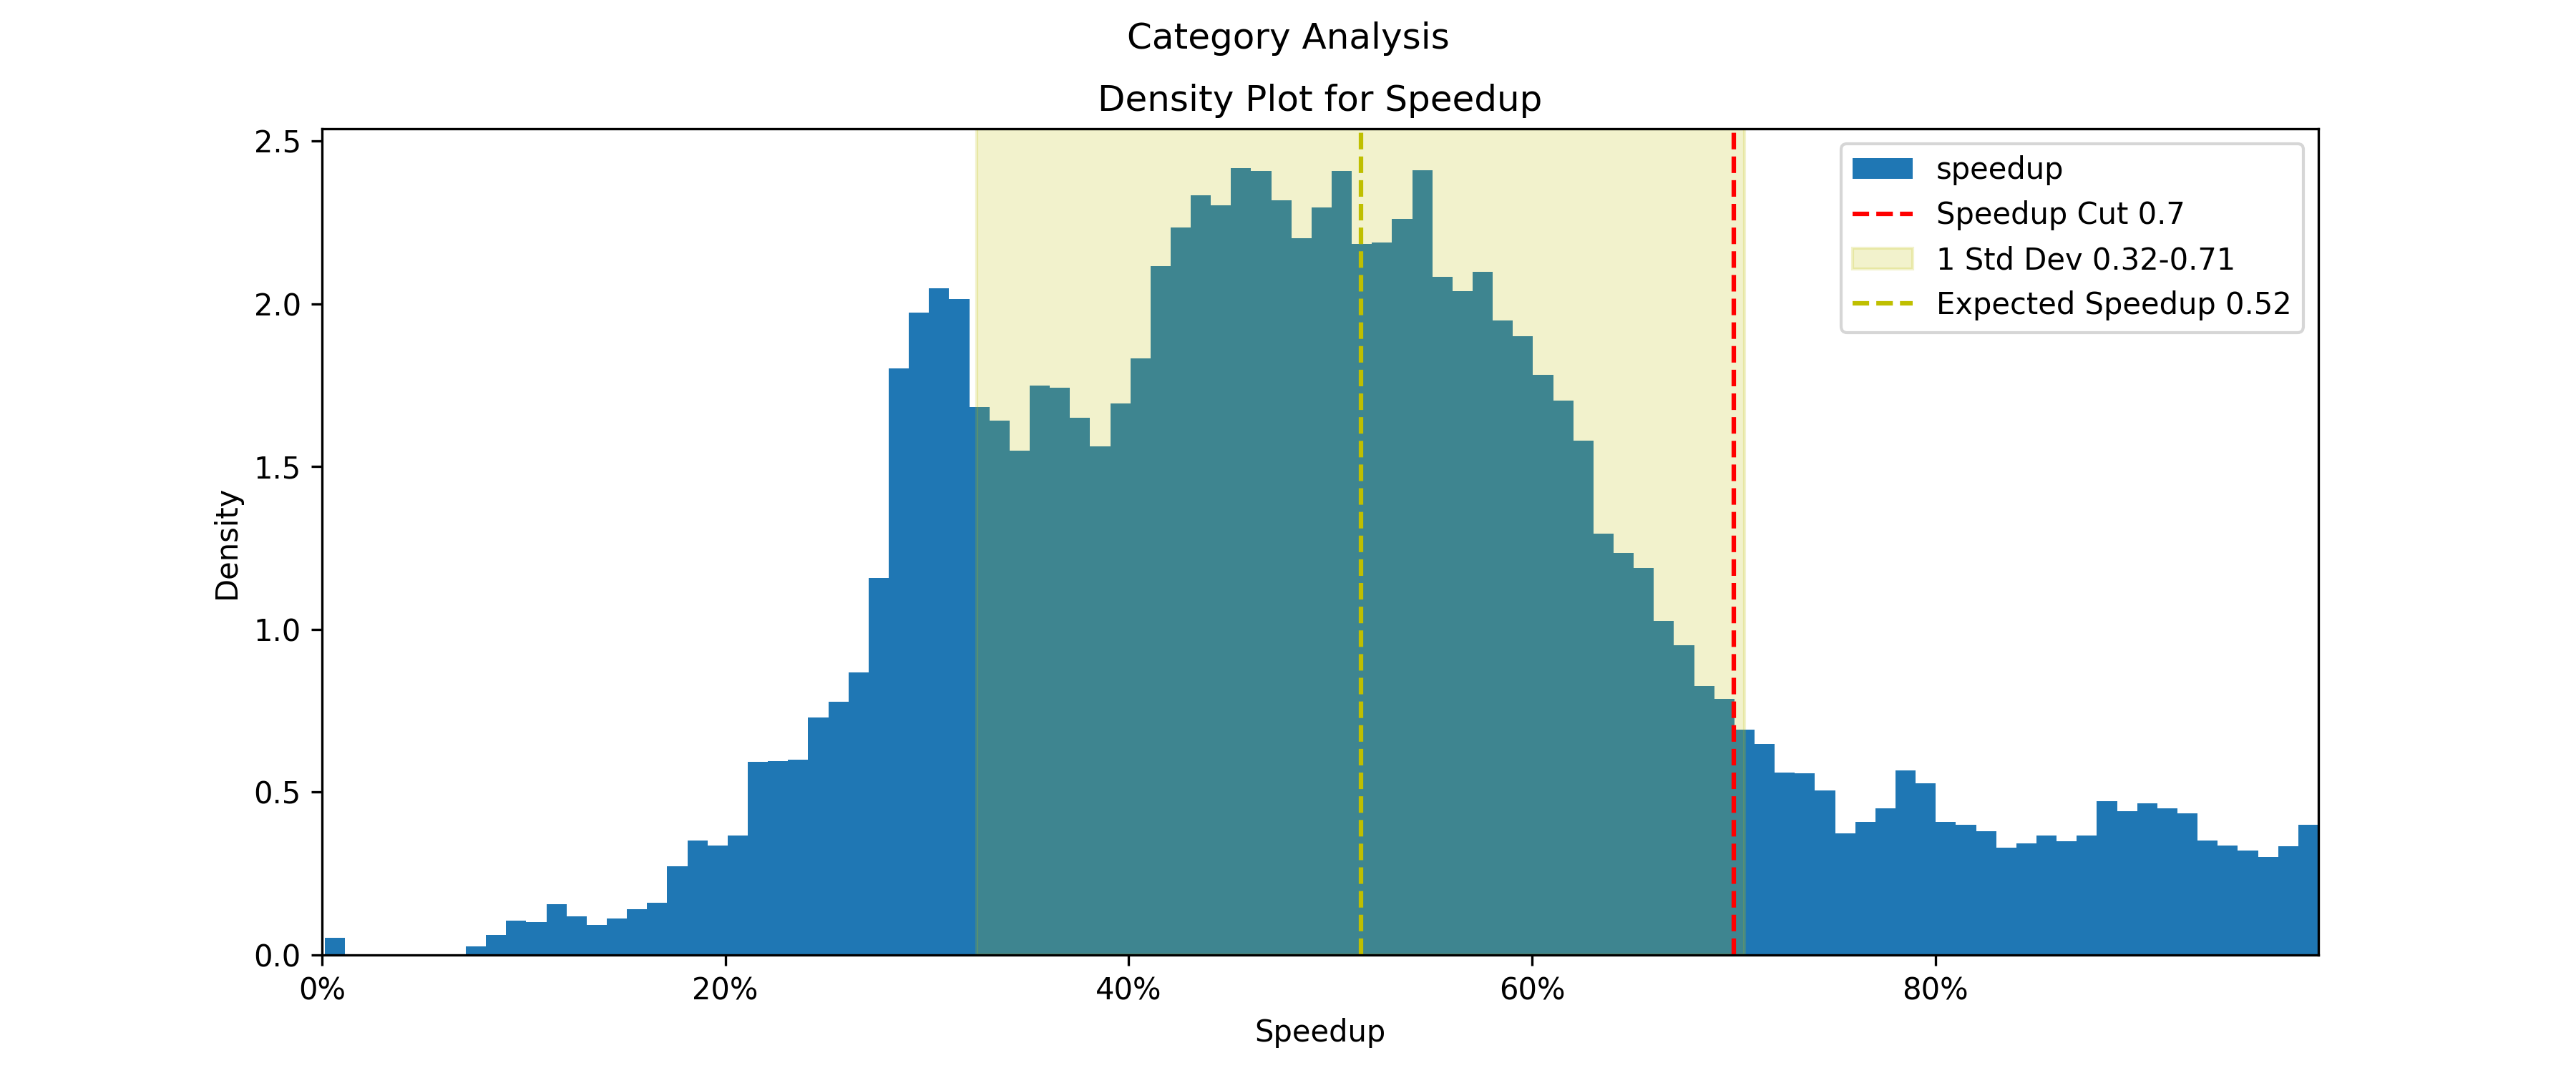
\includegraphics[width=1\textwidth]{figures/speedup.png}
	\end{figure}
\end{frame}

\begin{frame}
	\frametitle{Backup: Quality of Predictions}
	
	\begin{itemize}
		\item How well do tuning strategies suggest good configurations?
	\end{itemize}
	
	\begin{figure}
		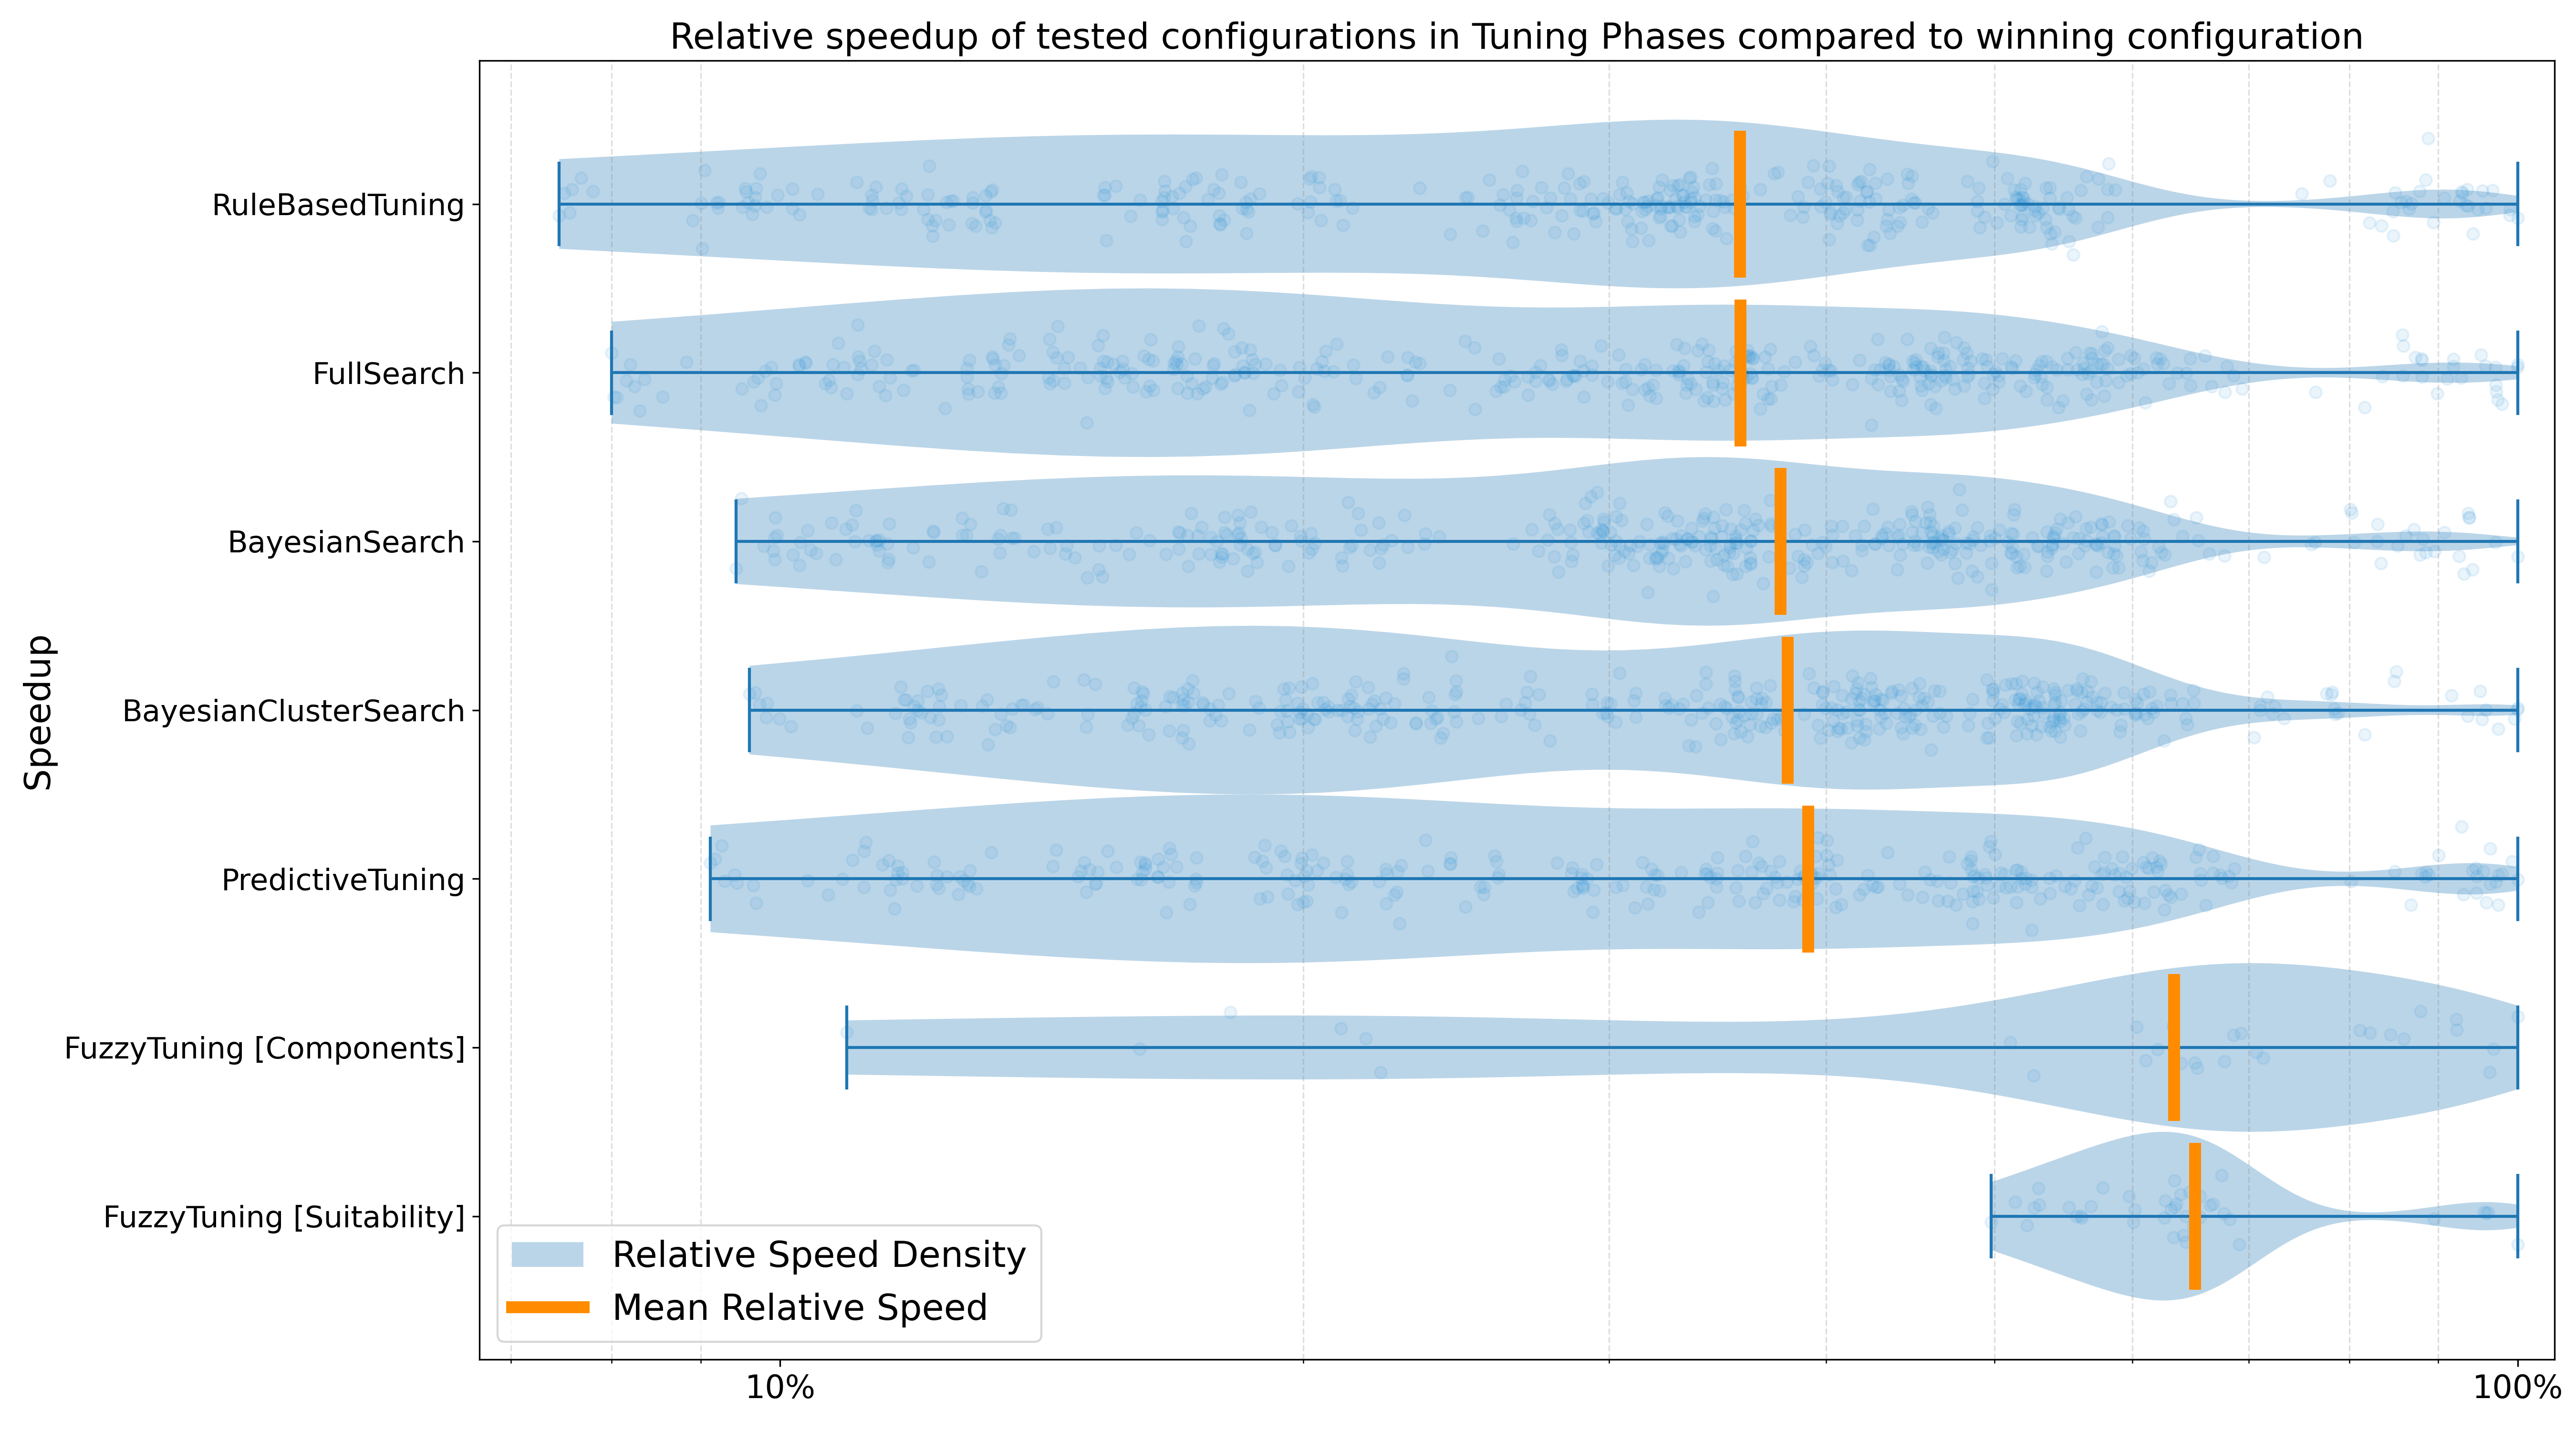
\includegraphics[width=0.8\paperwidth]{figures/prediction-quality.png}
	\end{figure}
	
\end{frame}

\begin{frame}
	\vspace{-0.8cm}
	\begin{figure}
		\centering
		\caption{\tiny{Source: \href{https://de.mathworks.com/help/fuzzy/fuzzy-inference-process.html}{MathWorks - Fuzzy Inference Process}}}
		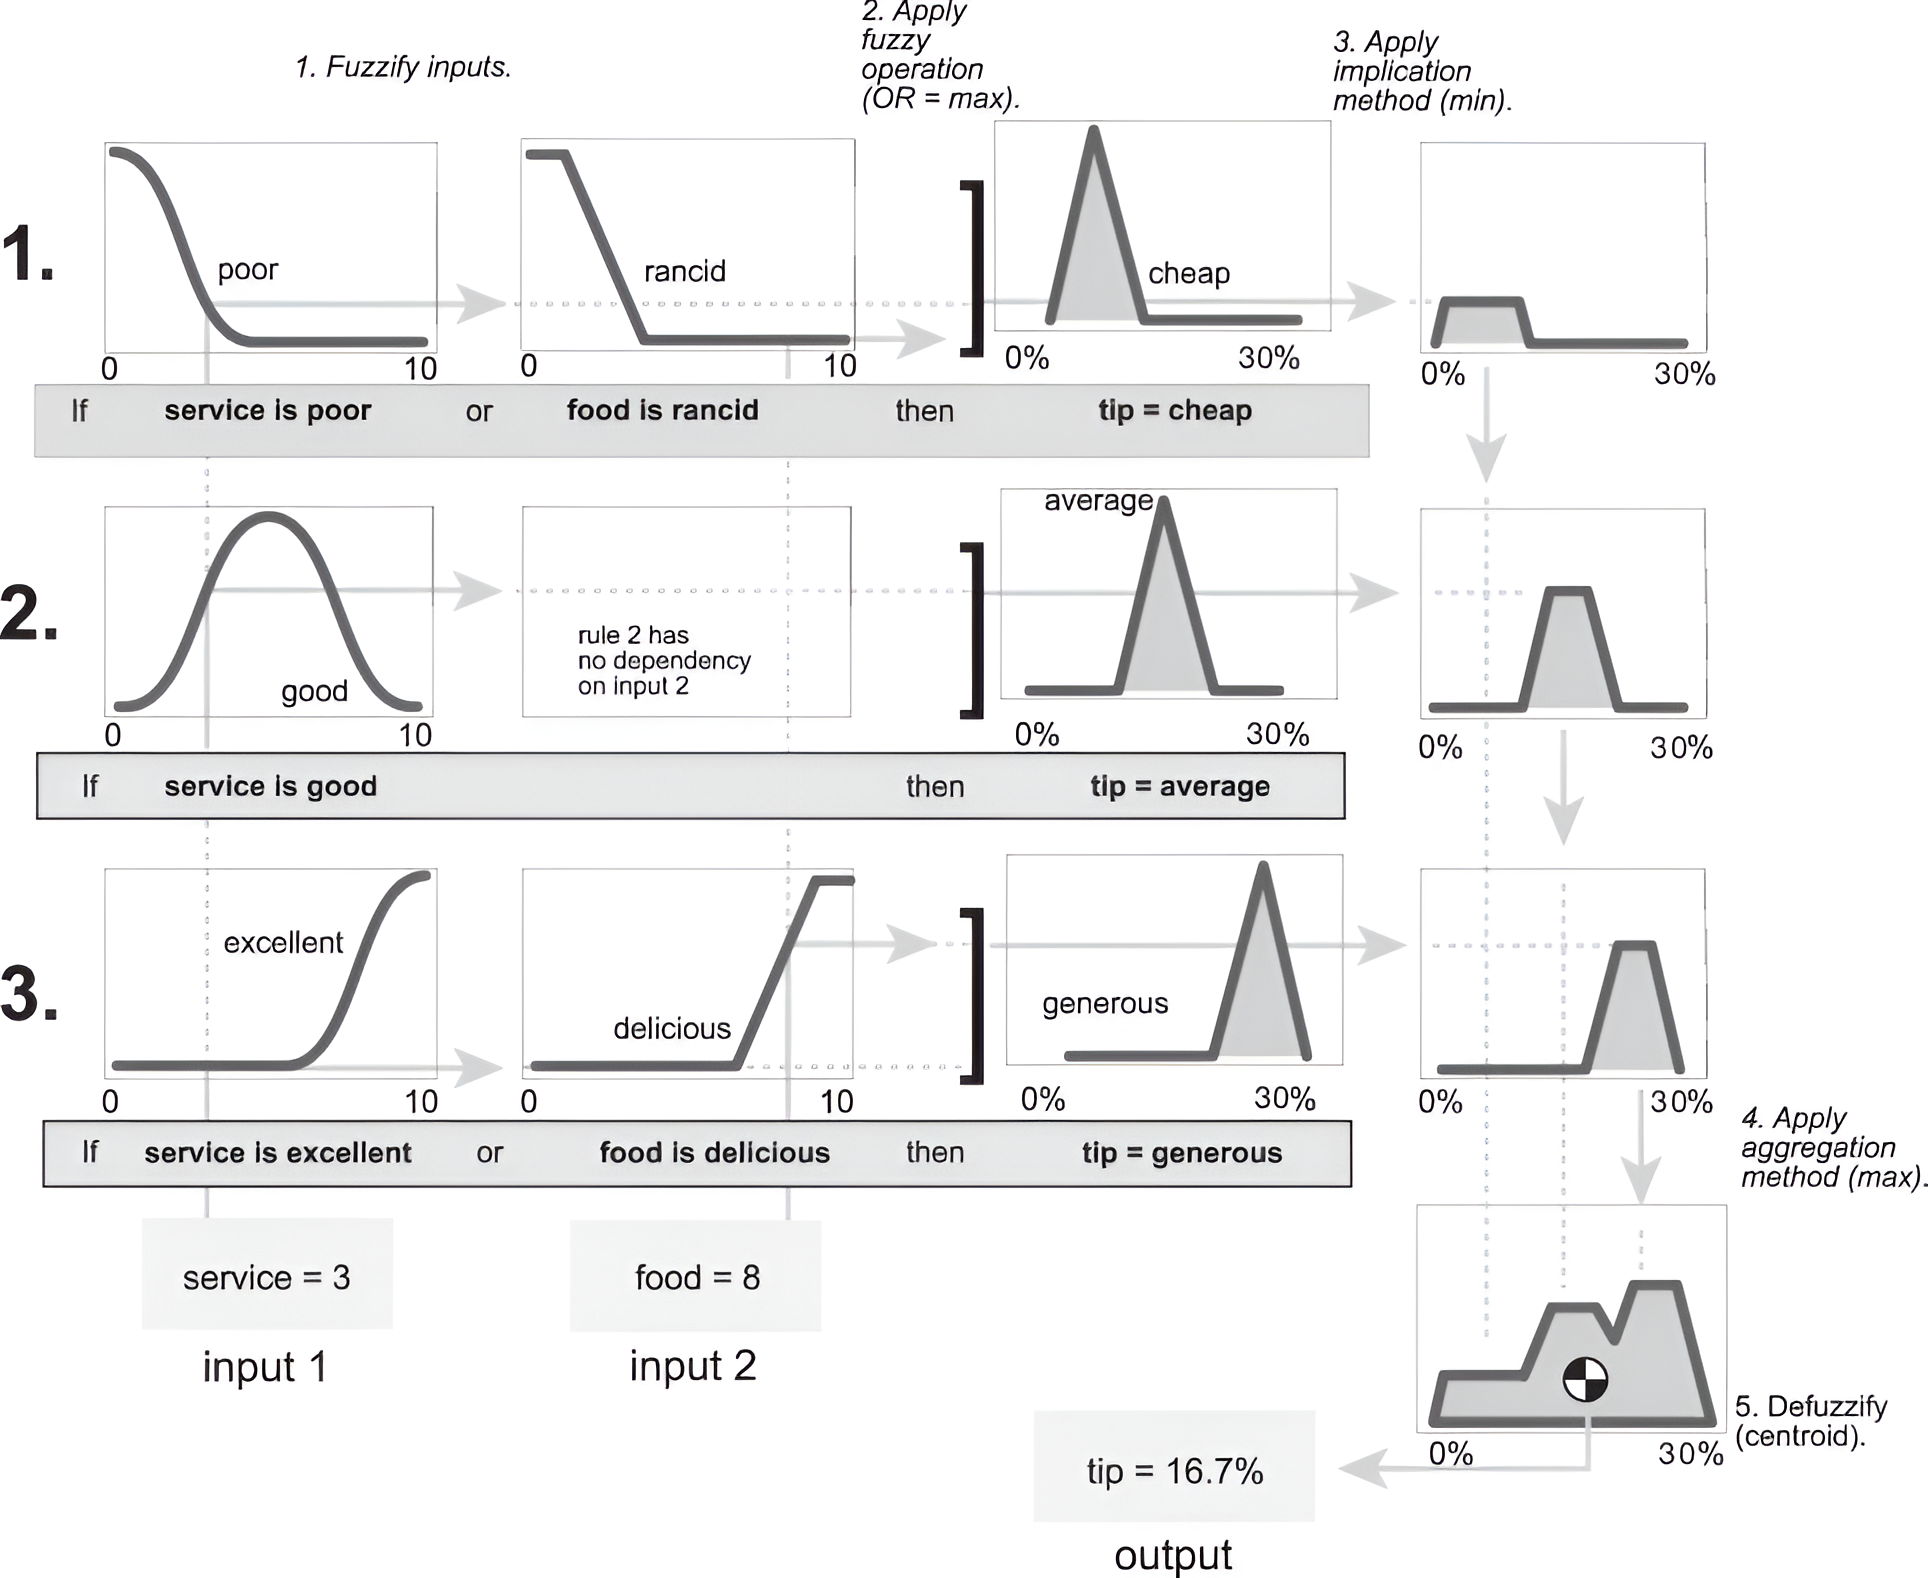
\includegraphics[width=0.8\paperwidth]{figures/FullInferenceProcess.png}
	\end{figure}
	\label{fig:fuzzy_inference_full}
	
\end{frame}


\end{document}
